% Chapter Template

\chapter{Experimental Results} % Main chapter title

\label{Chapter4} % Change X to a consecutive number; for referencing this chapter elsewhere, use \ref{ChapterX}

\lhead{Chapter 4. \emph{Experimental Results}} % Change X to a consecutive number; this is for the header on each page - perhaps a shortened title

%----------------------------------------------------------------------------------------
%	SECTION 1
%----------------------------------------------------------------------------------------

\section{The Model}

The most common form of representing a scale-free network is by using its degree of connections, where the horizontal axis represents number of connections, and the vertical axis represents the number of agents having that many connections.

\begin{figure}
\centering
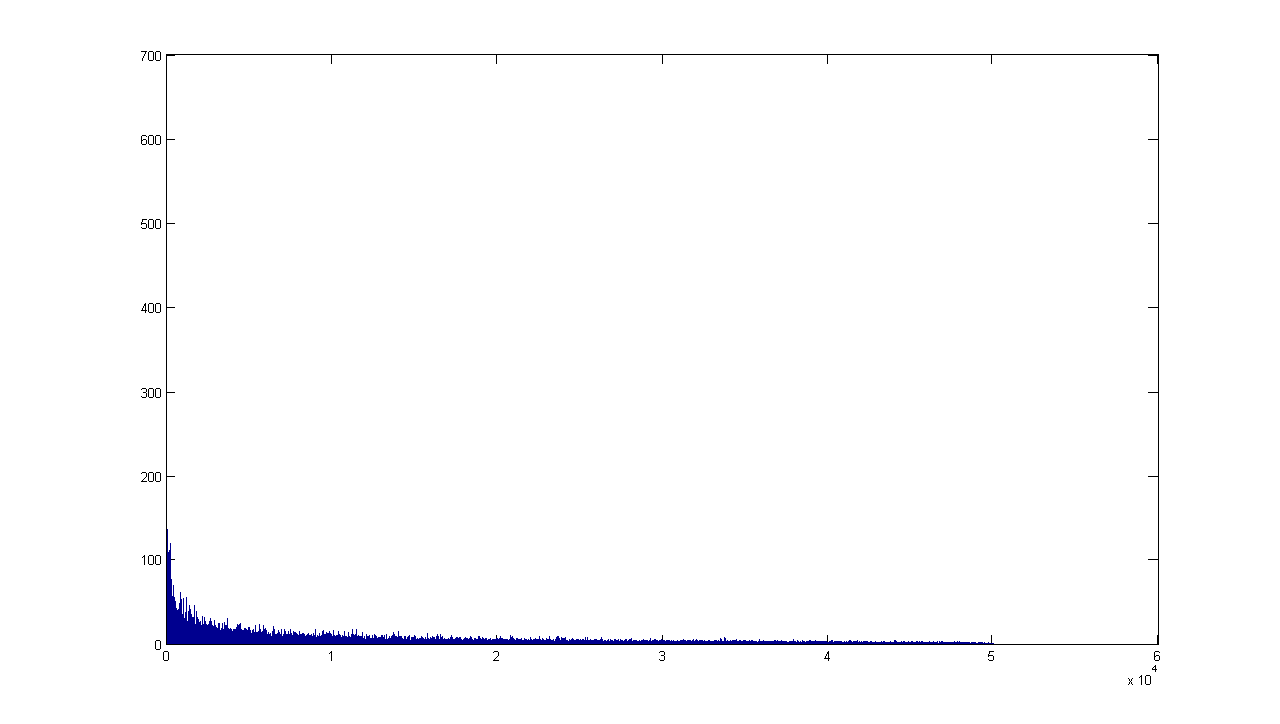
\includegraphics[scale=0.5]{Figures/50000m1_small_world}
\caption[Small World Network with Original Algorithm]{Small world Network, Original BA algorithm}
\label{fig:small_world_original}
\end{figure}

\begin{figure}
\centering
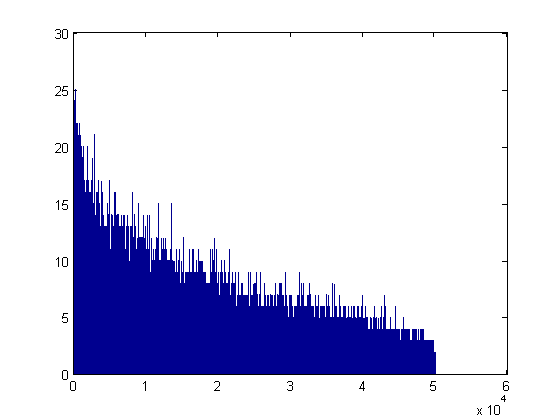
\includegraphics[scale=0.75]{Figures/50000m2_small_world}
\caption[Small World Network with Modified Algorithm]{Small world Network, Modified BA algorithm}
\label{fig:small_world_modified}
\end{figure}

Figures~\ref{fig:small_world_original} and ~\ref{fig:small_world_modified} show the different degrees in the connection in the case of using original BA algorithm and using our modified approach to the algorithm respectively.

It can be observed that using the constraint of `likemindedness' results in a drop in the horizontal axis values, which shows that lesser number of connections are formed.

The basic model was modified a lot with time, from the initial design, as the author learnt more. The development of the model can be explained in two parts.

%-----------------------------------
%	SUBSECTION 1
%-----------------------------------
\subsection{Small-World Networks}
Figures~\ref{fig:small_world_original} and ~\ref{fig:small_world_modified} both show discontinuation in the tail. 

On further inspection, it was found that the networks were displaying characterictics of Small-World networks~\cite{smallWorld}. The difference in what was required and what was achieved is made clear by Cohen \& Havlin~\cite{PhysRevLett.90.058701}.

This led to modifications in the design and the design explained in Chapter~\ref{Chapter3} was achieved.

%-----------------------------------
%	SUBSECTION 2
%-----------------------------------

\subsection{Scale-free Networks}

An example in comparison of both models, i.e., following original BA algorithm and the modified approach, can be seen in Figure~\ref{fig:scaleFree_comp}, where green color represents the original algorithm and blue represents the modified approach.

\begin{figure}
\centering
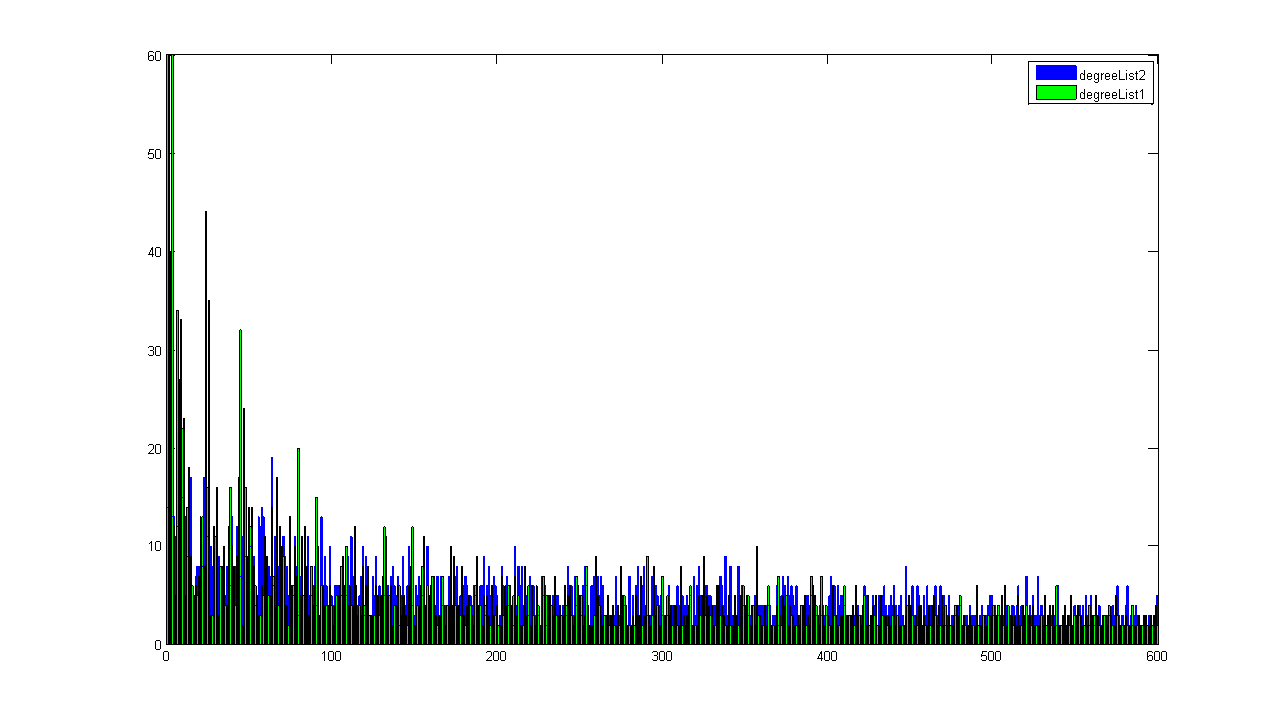
\includegraphics[scale=0.5]{Figures/scaleFree_comparison}
\caption[Comparison of Scale Free Networks]{Comparison of Scale Free Networks generated by the different algorithms for 1000 agents}
\label{fig:scaleFree_comp}
\end{figure}

These outputs were further tested for fit, using MATLAB's curve fitting toolbox, against a power-law curve, and the results are shown in figure~\ref{fig:power1} and ~\ref{fig:power2}.

\begin{figure}
\begin{center}$
\begin{array}{cc}
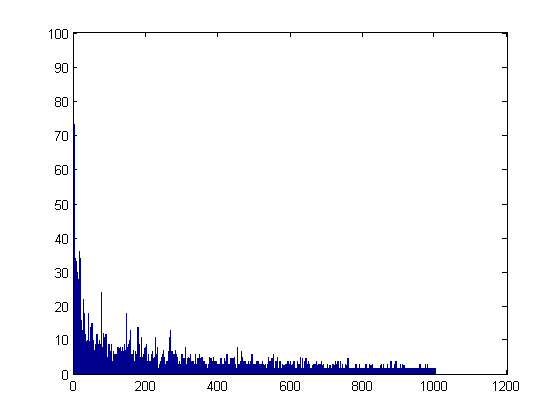
\includegraphics[scale=0.5]{Figures/1000m1} \\
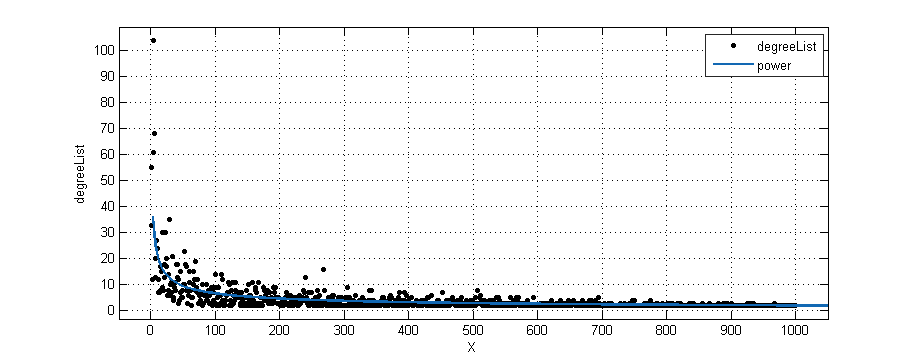
\includegraphics[scale=0.5]{Figures/1000m1_powerFit} 
\end{array}$
\end{center}
\caption[Power Law Fit for Original Algorithm]{Scale-Free network using BA algorithm and corresponding power law fit}
\label{fig:power1}
\end{figure}

\begin{figure}
\begin{center}$
\begin{array}{cc}
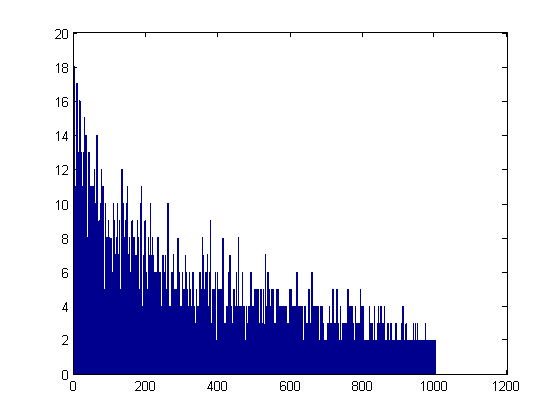
\includegraphics[scale=0.5]{Figures/1000m2} \\
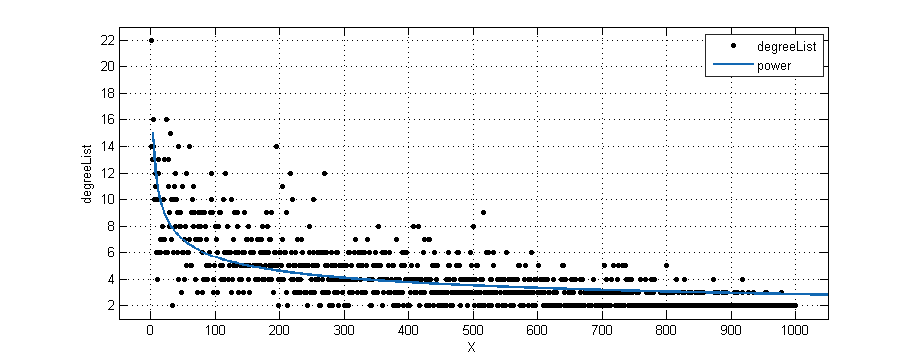
\includegraphics[scale=0.5]{Figures/1000m2_powerFit} 
\end{array}$
\end{center}
\caption[Power Law Fit for Modified Algorithm]{Scale-Free network using modified BA algorithm and corresponding power law fit}
\label{fig:power2}
\end{figure}


%----------------------------------------------------------------------------------------
%	SECTION 2
%----------------------------------------------------------------------------------------

\section{The Simulation}

The simulations resulted in three different types of outputs. They were all run for cases where on an average, every agent makes 3 connections. The different types of outputs are as follows:

\begin{enumerate}
\item[1] Color Histograms
\item[2] Spatial Clusters
\item[3] Cost-Gain Functions
\end{enumerate}

For the specific purposes of this thesis, spefically for analysis part, a particular set of `Gain' and `Cost' values, in accordance with the policies followed by the companies, were used. Keeping the gain for each influence fixed at `One' unit, and allowing the agents to move 0.2 percent of the distance at a single step, the costs are varied as per table~\ref{table:cost}.

The costs are also equal to the effort, i.e., the amount of fraction of distance travelled by the company towards the agent.

\begin{table}
\begin{center}
\begin{tabular}{|l||c|r|}
\hline
caseId & cost1 & cost2 \\ \hline 
Base1 & 0.001 & 0.001 \\ 
Base2 & 0.002 & 0.002 \\
Base3 & 0.01 & 0.01 \\
Base4 & 0.02 & 0.02 \\
Diff1 & 0.001 & 0.002 \\
Diff2 & 0.001 & 0.01 \\
Diff3 & 0.001 & 0.02 \\
Diff4 & 0.002 & 0.01 \\
Diff5 & 0.002 & 0.02 \\
Diff6 & 0.01 & 0.02 \\
\hline
\end{tabular} 
\caption[Cost ]{Costs for various cases for both the companies}
\label{table:cost}
\end{center}
\end{table}

%-----------------------------------
%	SUBSECTION 1
%-----------------------------------
\subsection{Color Histograms}

These histograms give the observer a good view of how the agents tend to lean from one company towards another.

Since the network has a large concentration of agents initially seeded to a neutral color which is equidistant from both company1 and company2, it could be observed that a huge initial spike is in the center, while the two companies in question are at the extreme corners.

The change in the heights of different columns can be seen in fig.~\ref{fig:cluster1}. The horizontal axis represents the color value, and the vertical axis represents the number of agents having that value for the color attribute, or, in other terms, the membership of that company.

Fig.~\ref{fig:cluster2} shows a similar output for 10000 agents. This case shows that although the agents move away from the central, equidistant clusters, they may not always reach all the way to either of the company clusters. This is evident by the change of height of the intermediate columns.

\begin{figure}
\begin{center}$
\begin{array}{cc}
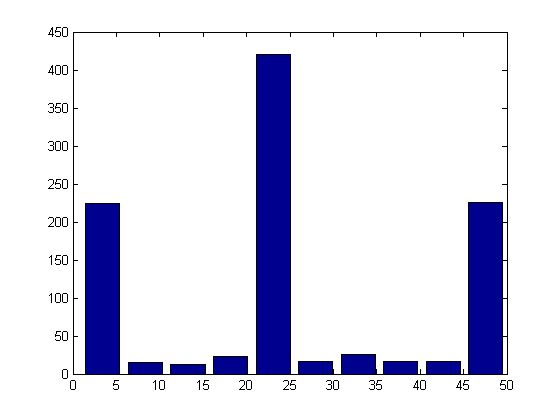
\includegraphics[scale=0.5]{Figures/1000_m2_initial}
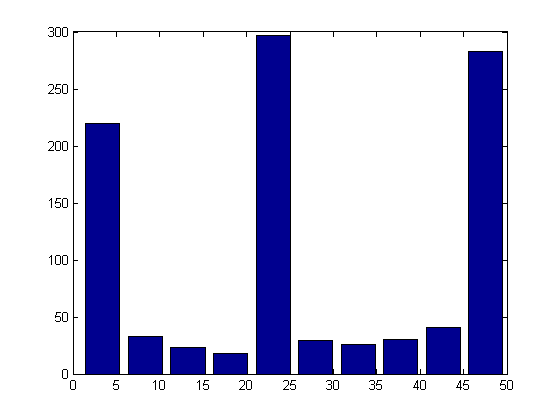
\includegraphics[scale=0.5]{Figures/1000_m2_final} 
\end{array}$
\end{center}
\caption[Color Clusters 1]{Color Clusters for 1000 agents. Initial Cluster on left, and final clusters on right.}
\label{fig:cluster1}
\end{figure}

\begin{figure}
\begin{center}$
\begin{array}{cc}
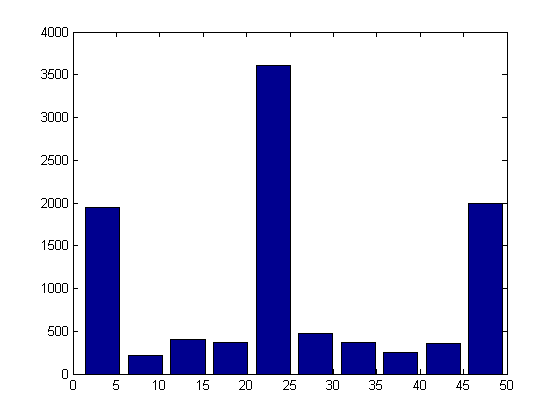
\includegraphics[scale=0.5]{Figures/10000_m2_initial}
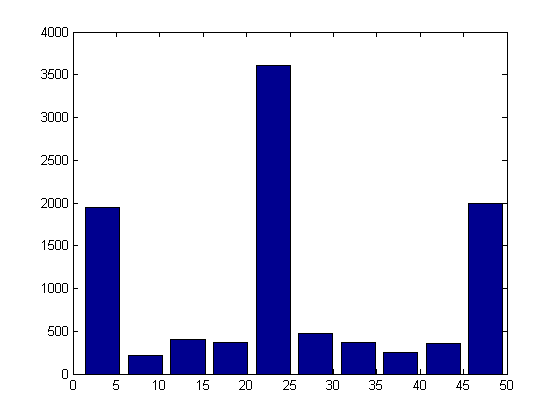
\includegraphics[scale=0.5]{Figures/10000_m2_final} 
\end{array}$
\end{center}
\caption[Color Clusters 2]{Color Clusters for 10000 agents. Initial Cluster on left, and final clusters on right.}
\label{fig:cluster2}
\end{figure}


%-----------------------------------
%	SUBSECTION 2
%-----------------------------------

\subsection{Spatial Cluster}

As mentioned in chapter~\ref{Chapter2}, section~\ref{sec:presentaion}, these outputs were necessary to visualise the cost incurred to the companies.
 
The three dimensions of any element of these plots are its x-y coordinates and its color. The agents are visible as `o' markers, while the companies are shown with `*' markers.

The simulation allows the observer to see the agents change their color as they move towards a specific company. Some screenshots of the simulations can be seen in fig.~\ref{fig:spatial1} and ~\ref{fig:spatial2}.

While fig.~\ref{fig:spatial1} is easier on the human-eye, fig.~\ref{fig:spatial2} is a result of a lot more iterations and is richer in terms of analytics.

\begin{figure}
\begin{center}$
\begin{array}{cc}
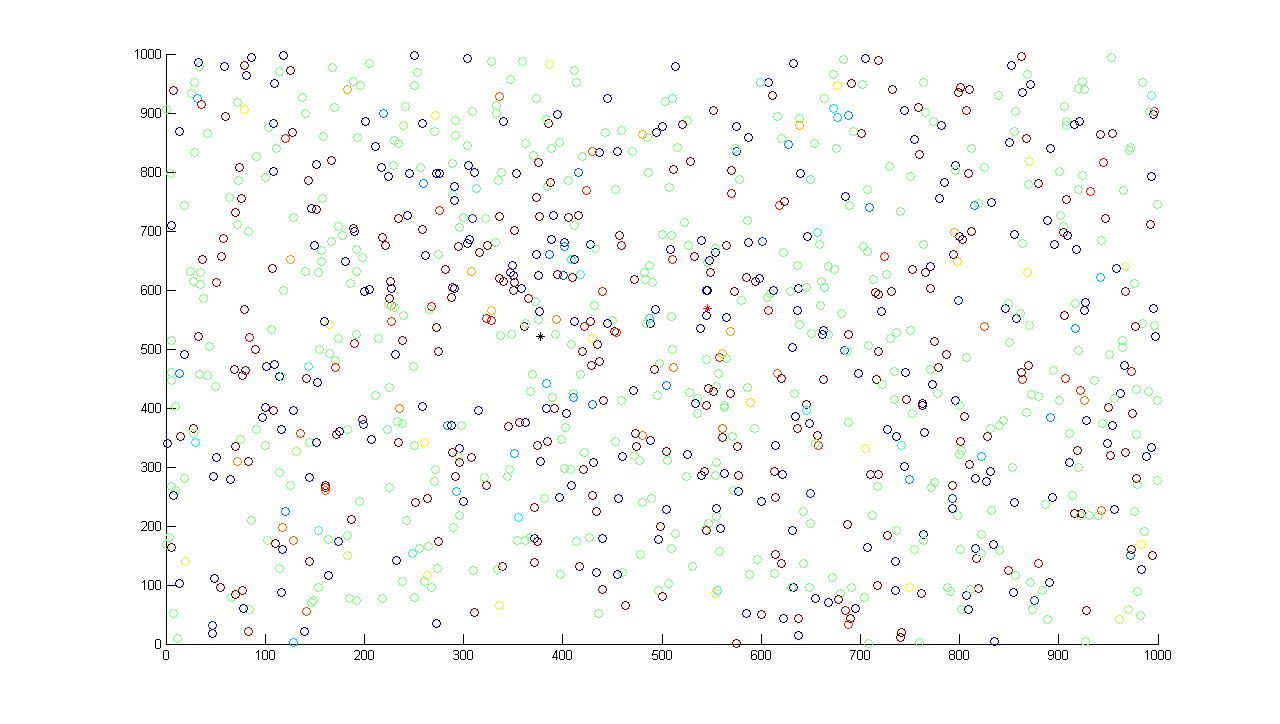
\includegraphics[scale=0.25]{Figures/1000_m2_initial_spatial}
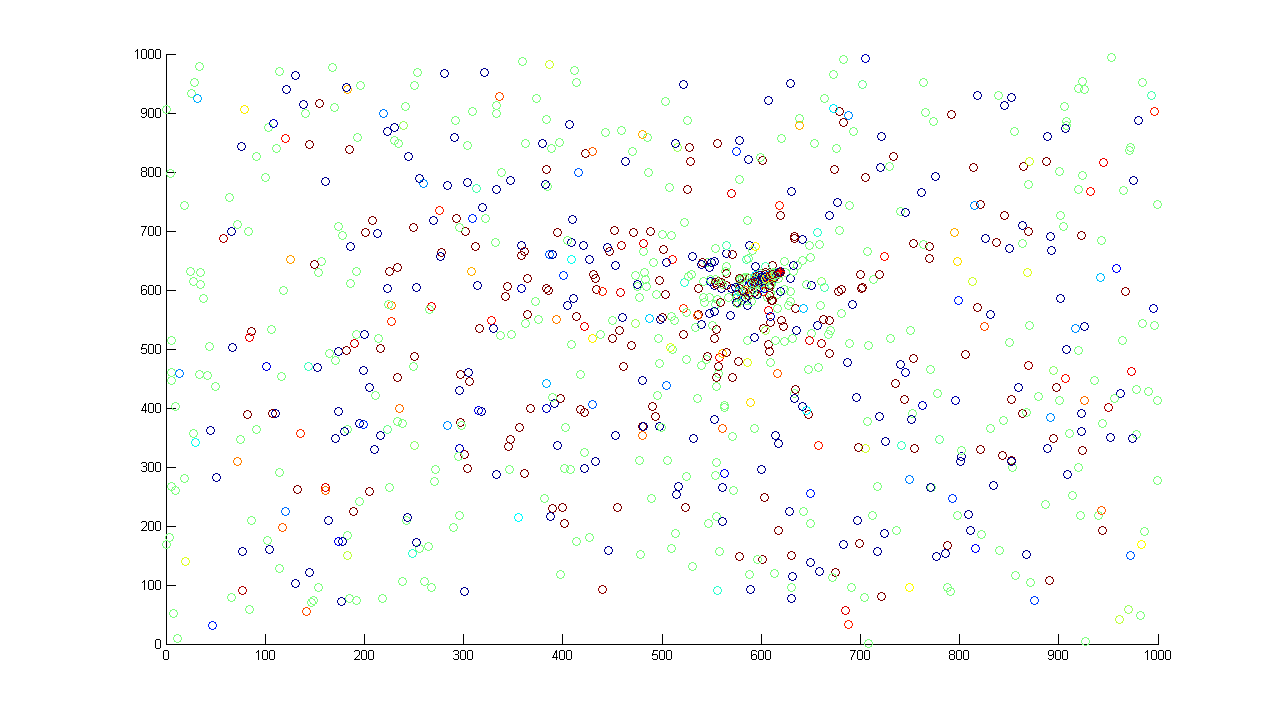
\includegraphics[scale=0.25]{Figures/1000_m2_final_spatial} 
\end{array}$
\end{center}
\caption[Spatial Clusters 1]{Spatial Clusters for 1000 agents. Initial Cluster on left, and final clusters on right.}
\label{fig:spatial1}
\end{figure}


\begin{figure}
\begin{center}$
\begin{array}{cc}
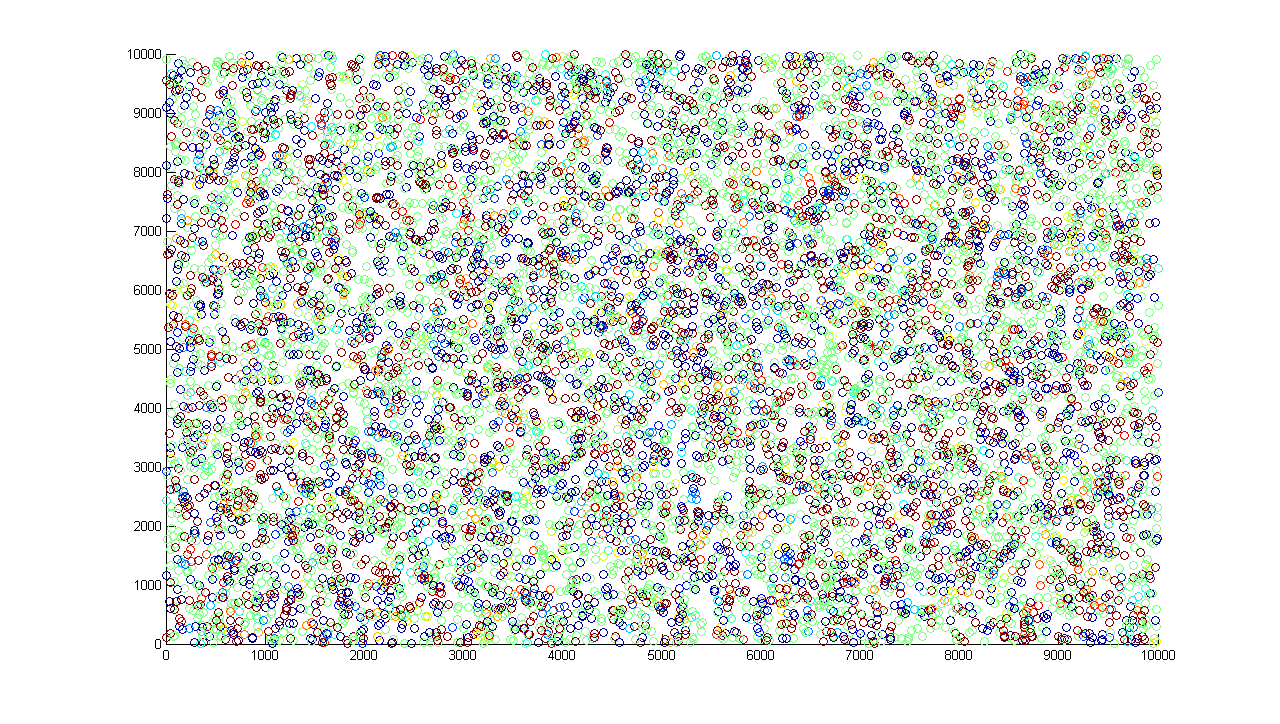
\includegraphics[scale=0.25]{Figures/10000_m2_initial_spatial}
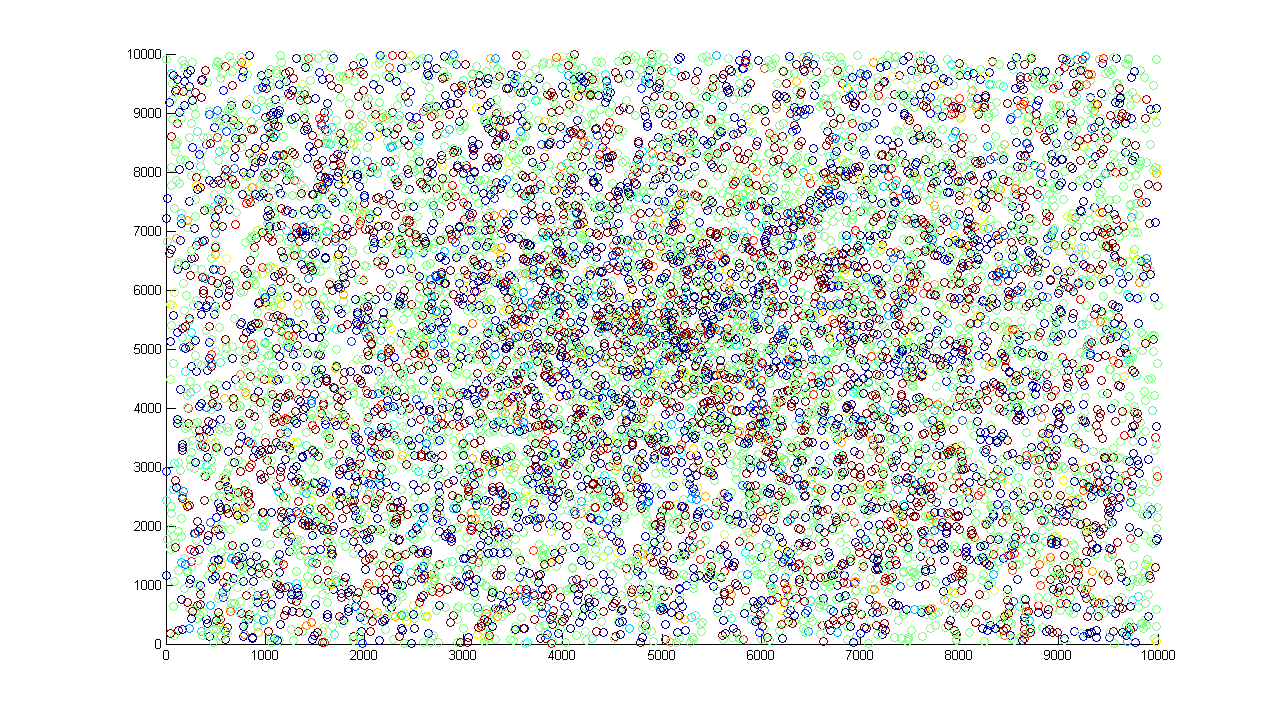
\includegraphics[scale=0.25]{Figures/10000_m2_final_spatial} 
\end{array}$
\end{center}
\caption[Spatial Clusters 2]{Spatial Clusters for 10000 agents. Initial Cluster on left, and final clusters on right.}
\label{fig:spatial2}
\end{figure}


%-----------------------------------
%	SUBSECTION 3
%-----------------------------------

\subsection{Cost-Gain Function}
\label{sec:cost_gain}
The simulation keeps track of the cost and gain for each company according to table~\ref{table:cost}. Company1 follows cost1 while company2 follows cost2, and the caseId tells us about the relation in the policies.

The generic spread and the population count of the companies was monitored, and they tend to show exponential nature of change.

\begin{figure}
\begin{center}$
\begin{array}{cc}
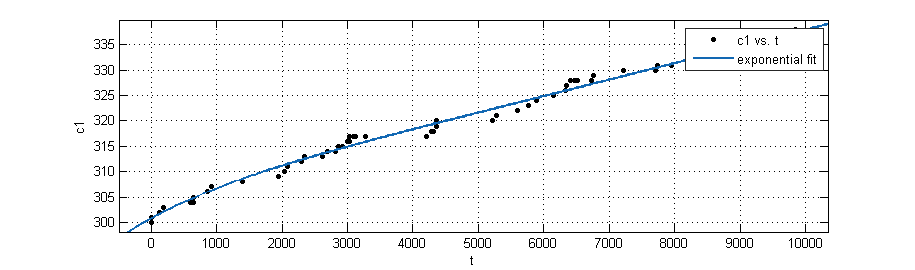
\includegraphics[scale=0.5]{Figures/diffusionTracking_exponentialFit_1000} \\
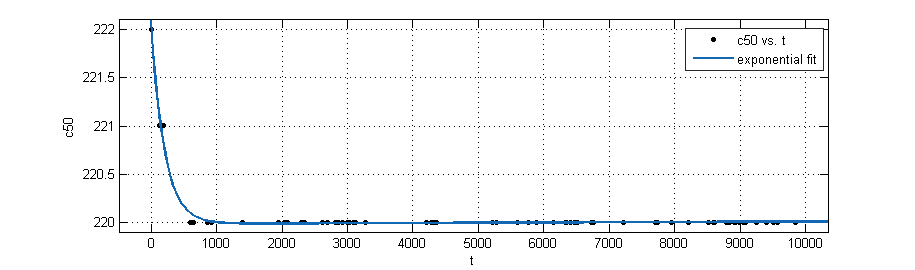
\includegraphics[scale=0.5]{Figures/diffusionTracking_exponentialFit_1000_decrease} 
\end{array}$
\end{center}
\caption[Diffusion 1]{Changes in membership of company for 1000 agents }
\label{fig:diffusion1}
\end{figure}

\begin{figure}
\begin{center}$
\begin{array}{cc}
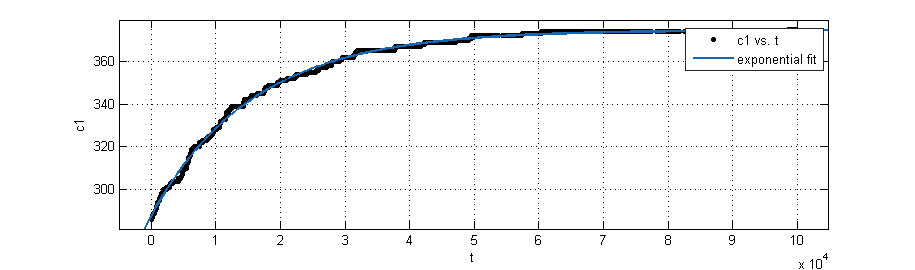
\includegraphics[scale=0.5]{Figures/diffusionTracking_exponentialFit_10000} \\
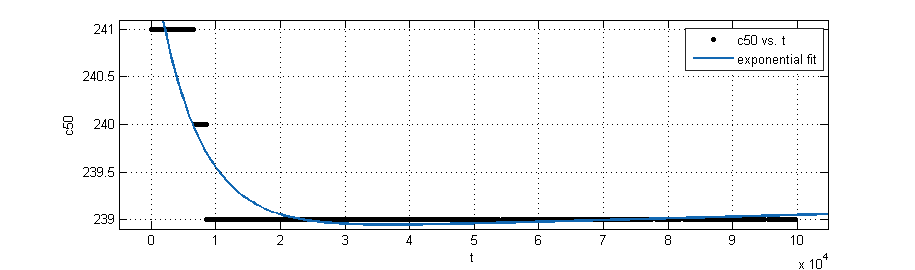
\includegraphics[scale=0.5]{Figures/diffusionTracking_exponentialFit_10000_decrease} 
\end{array}$
\end{center}
\caption[Diffusion 2]{Changes in membership of company for 10000 agents }
\label{fig:diffusion2}
\end{figure} 

Fig.~\ref{fig:diffusion1} and ~\ref{fig:diffusion2} show the increase and decrease of the membership of the companies against exponential fit. The x-axis represents time steps while the y-axis shows the membership value of a cluster, representing the number of agents fully believing in the company.

The cases from table~\ref{table:cost} show the functions in the form of equation~\ref{eqn:cost_gain}. The graphs presented here demonstrate the overall gain for Company2 relative to Company1, changing with time steps along the x-axis. These results can be divided into two categories. These are :

\begin{enumerate}
\item[1] \emph{Base} cases

These cases see both companies taking equal cost, and are meant to give the observer an idea about behaviour of both companies under similar policies. The output of these cases can be seen in fig.~\ref{fig:base1},~\ref{fig:base2},~\ref{fig:base3}, and ~\ref{fig:base4}.

\item[2] \emph{Diff} cases
These cases witness the companies following different policies, and allows the observer to analyse the policies. In this approach, cost for Company1 is kept at a constant while the cost for Company2 is increased, and the observed results are recorded. 
The output of these cases can be seen in fig.~\ref{fig:diff1}, ~\ref{fig:diff2}, ~\ref{fig:diff3}, ~\ref{fig:diff4}, ~\ref{fig:diff5}, and ~\ref{fig:diff6}. 

\end{enumerate}

\begin{figure}
\begin{center}$
\begin{array}{ccc}
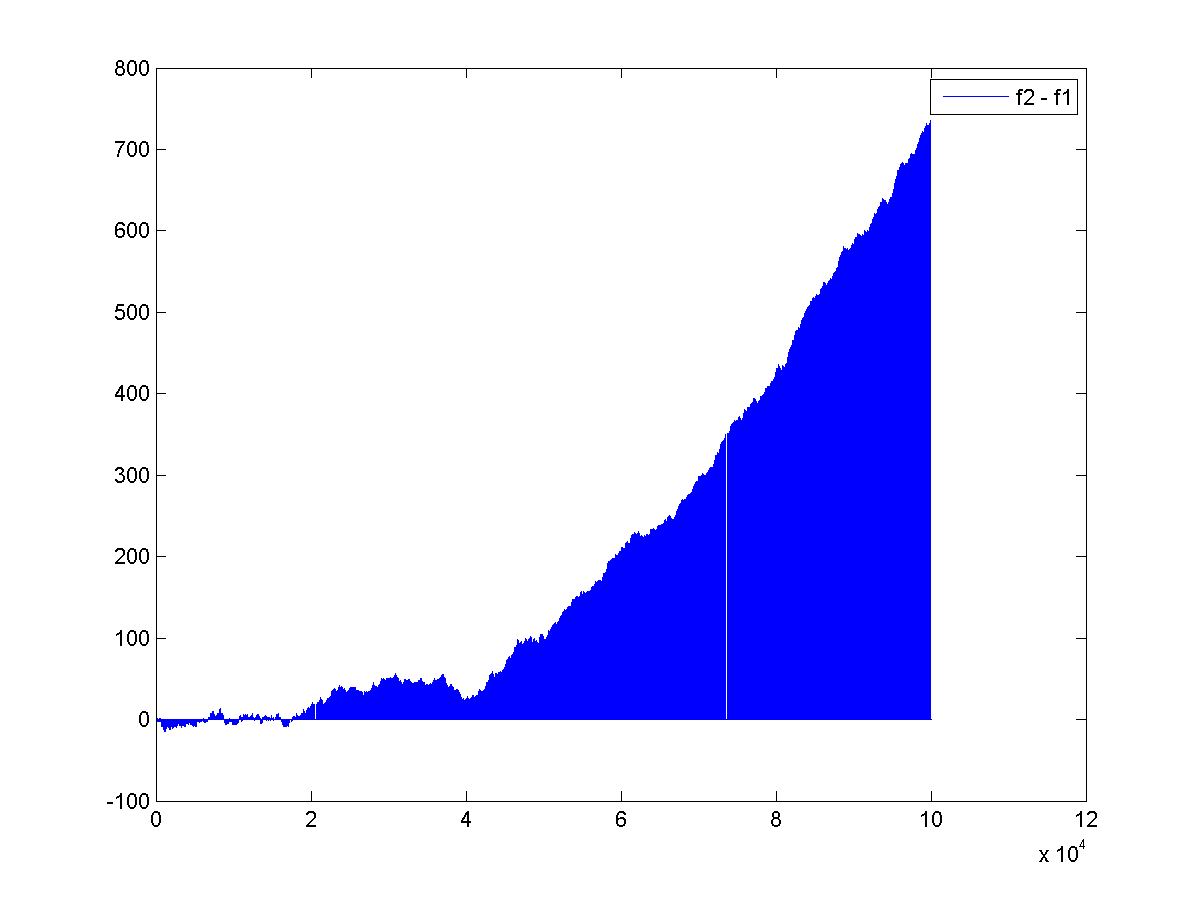
\includegraphics[scale=0.33]{Figures/base1/base1_1} 
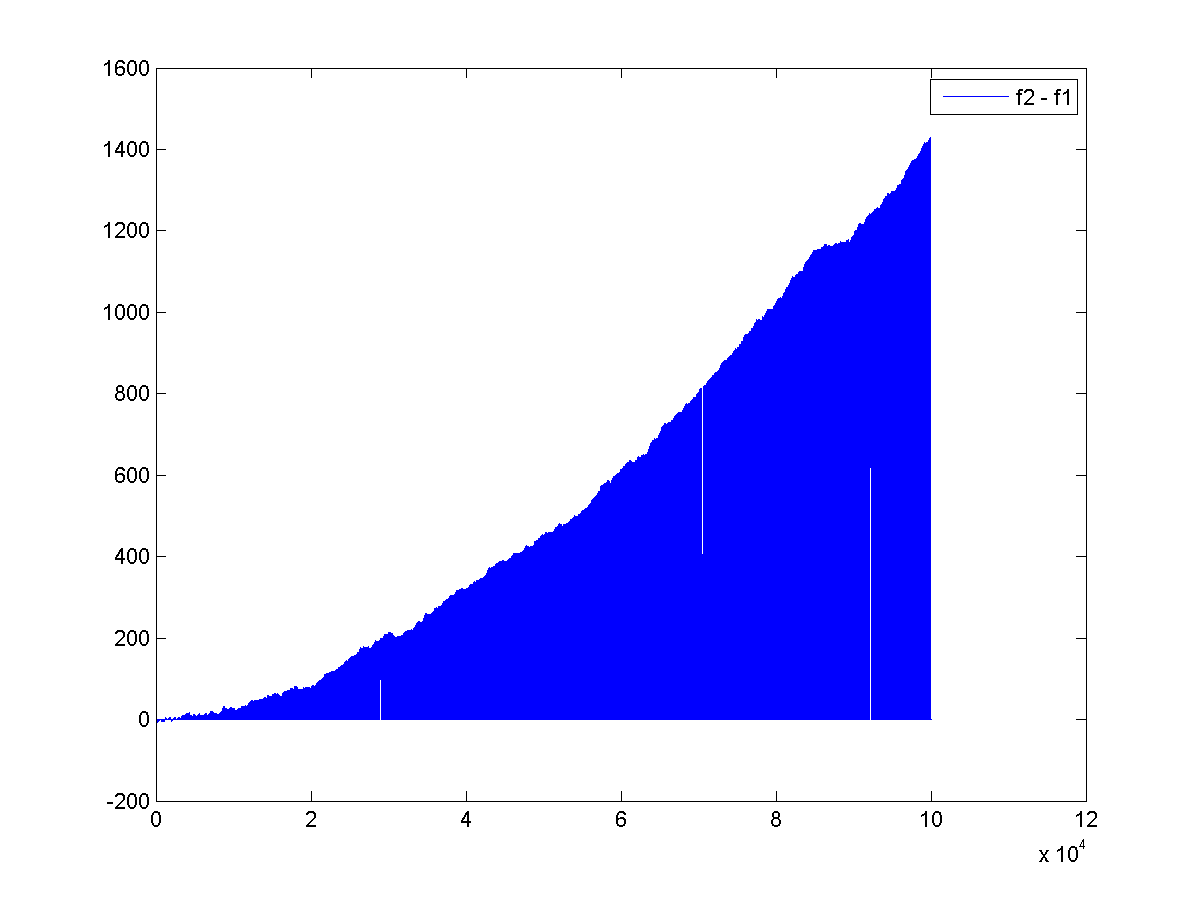
\includegraphics[scale=0.33]{Figures/base1/base1_2} \\
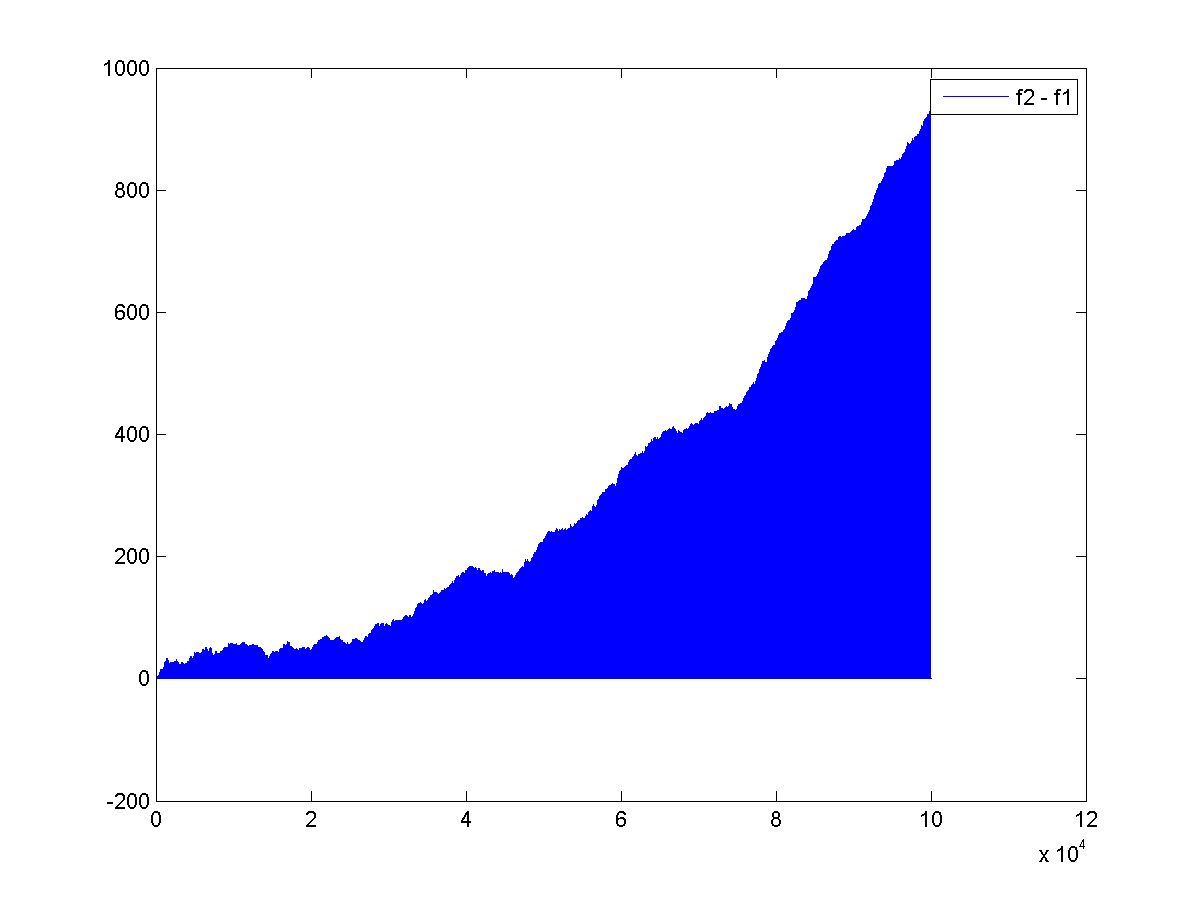
\includegraphics[scale=0.33]{Figures/base1/base1_3}
\end{array}$
\end{center}
\caption[Base case 1]{Results from three simulations for base case 1.}
\label{fig:base1}
\end{figure}

\begin{figure}
\begin{center}$
\begin{array}{ccc}
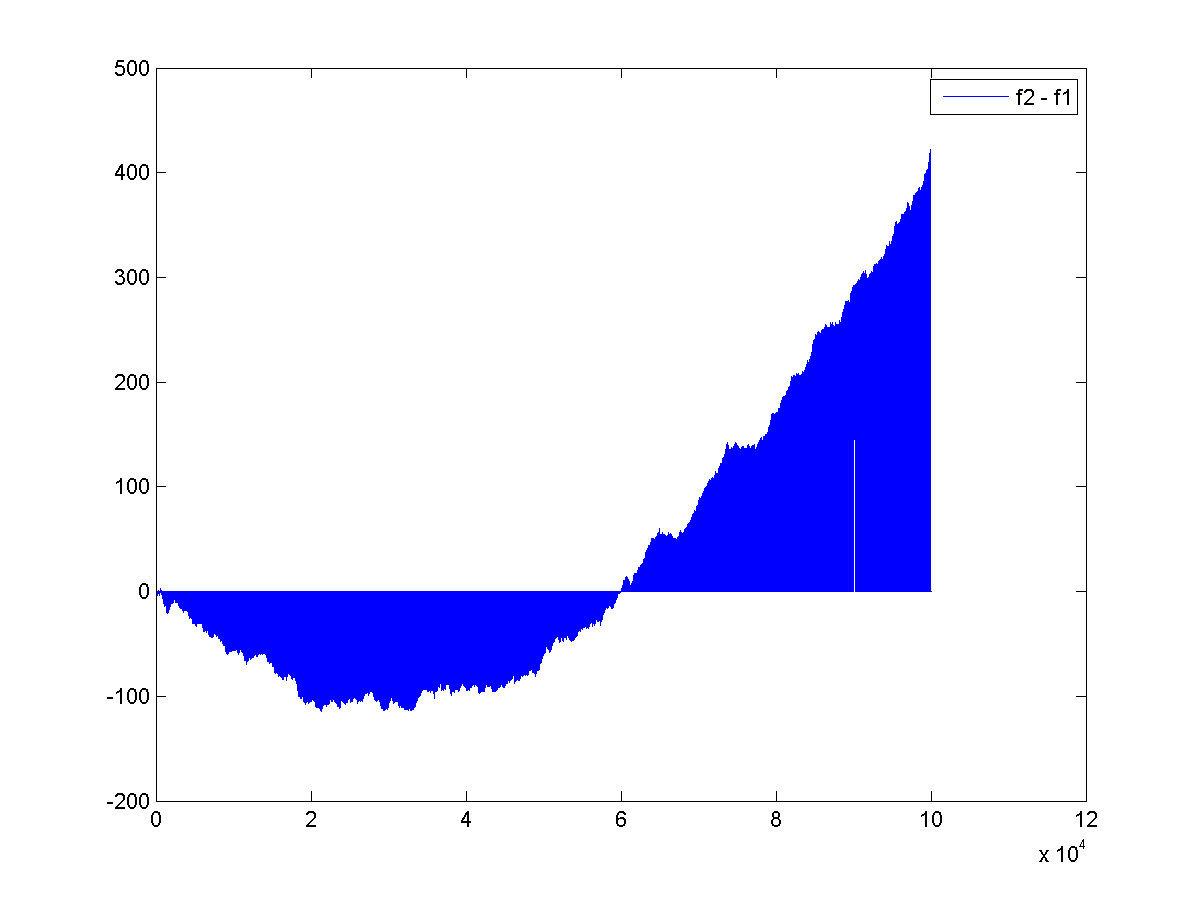
\includegraphics[scale=0.33]{Figures/base1/base2_1} 
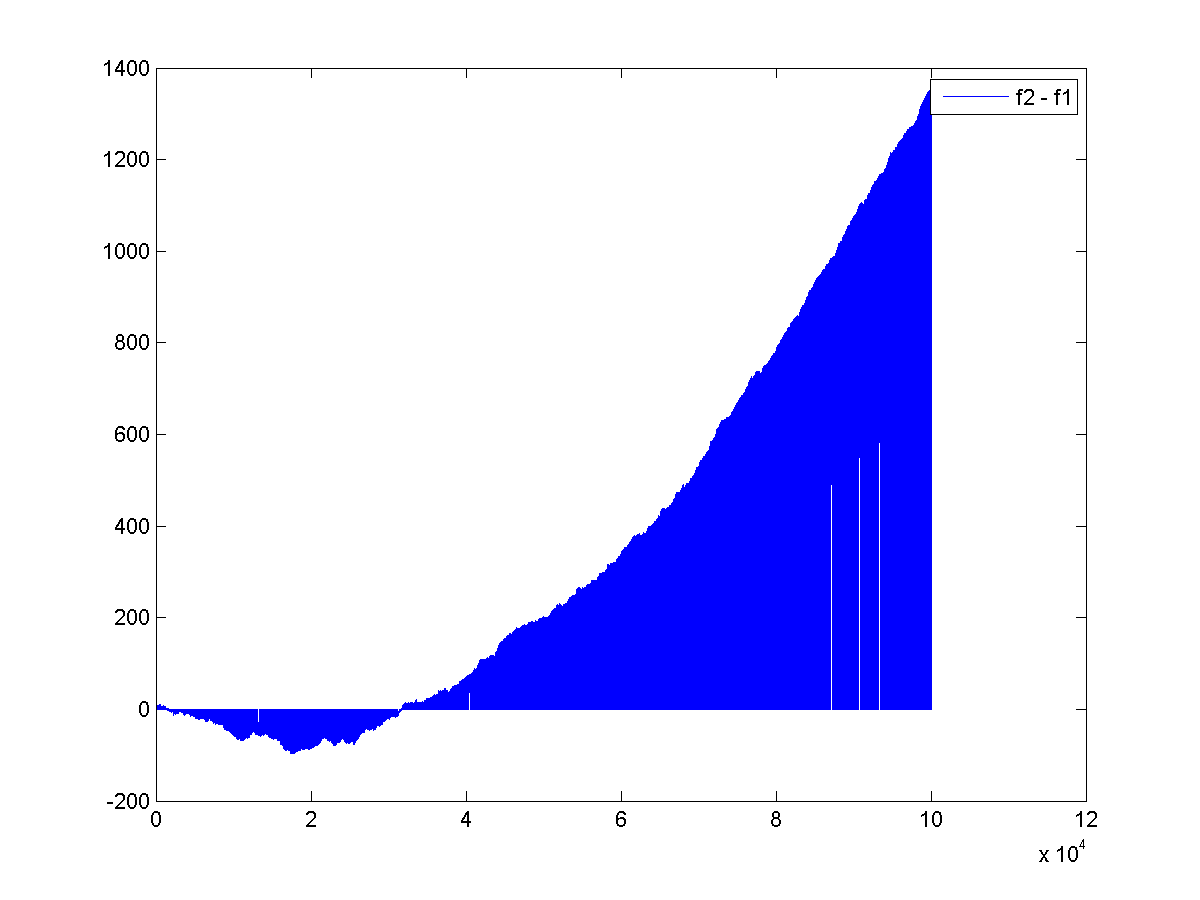
\includegraphics[scale=0.33]{Figures/base1/base2_2} \\
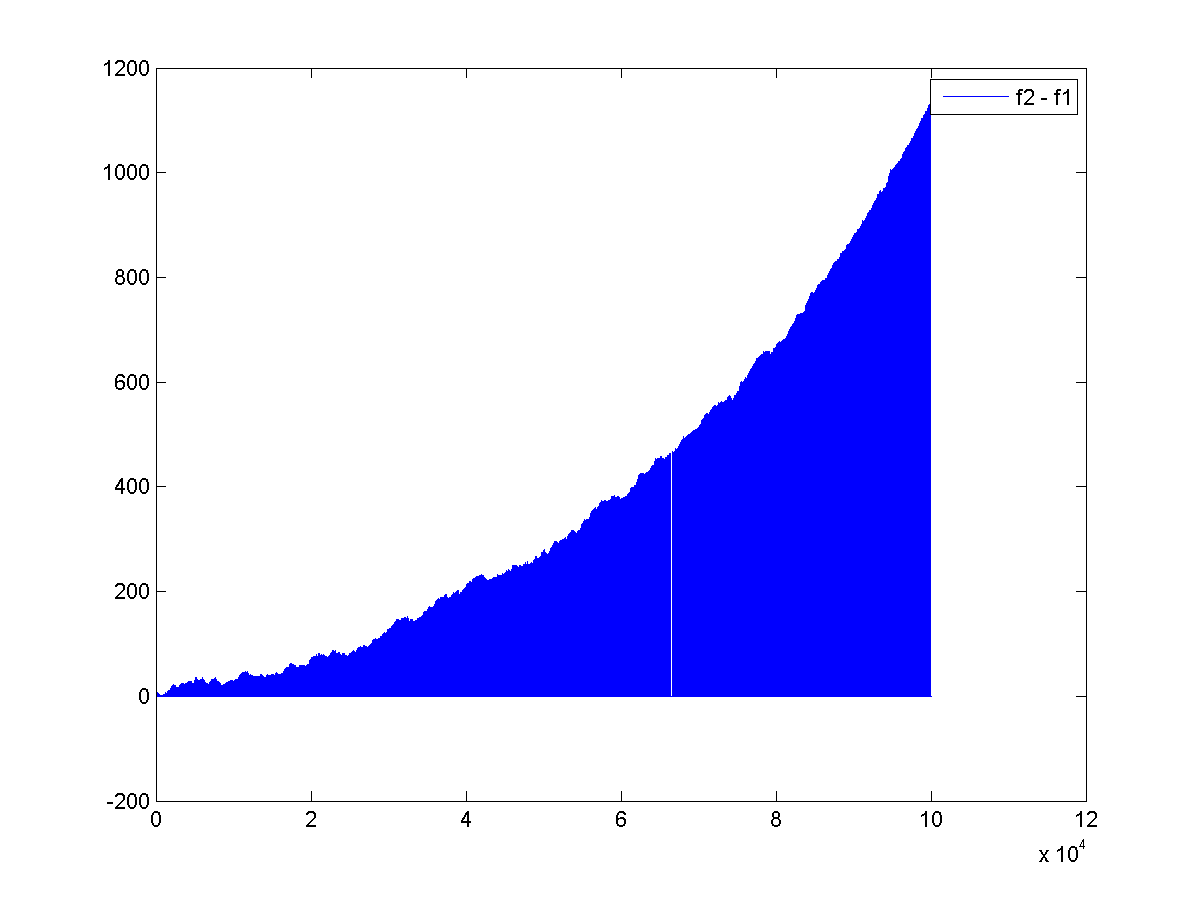
\includegraphics[scale=0.33]{Figures/base1/base2_3}
\end{array}$
\end{center}
\caption[Base case 2]{Results from three simulations for base case 2.}
\label{fig:base2}
\end{figure}

\begin{figure}
\begin{center}$
\begin{array}{ccc}
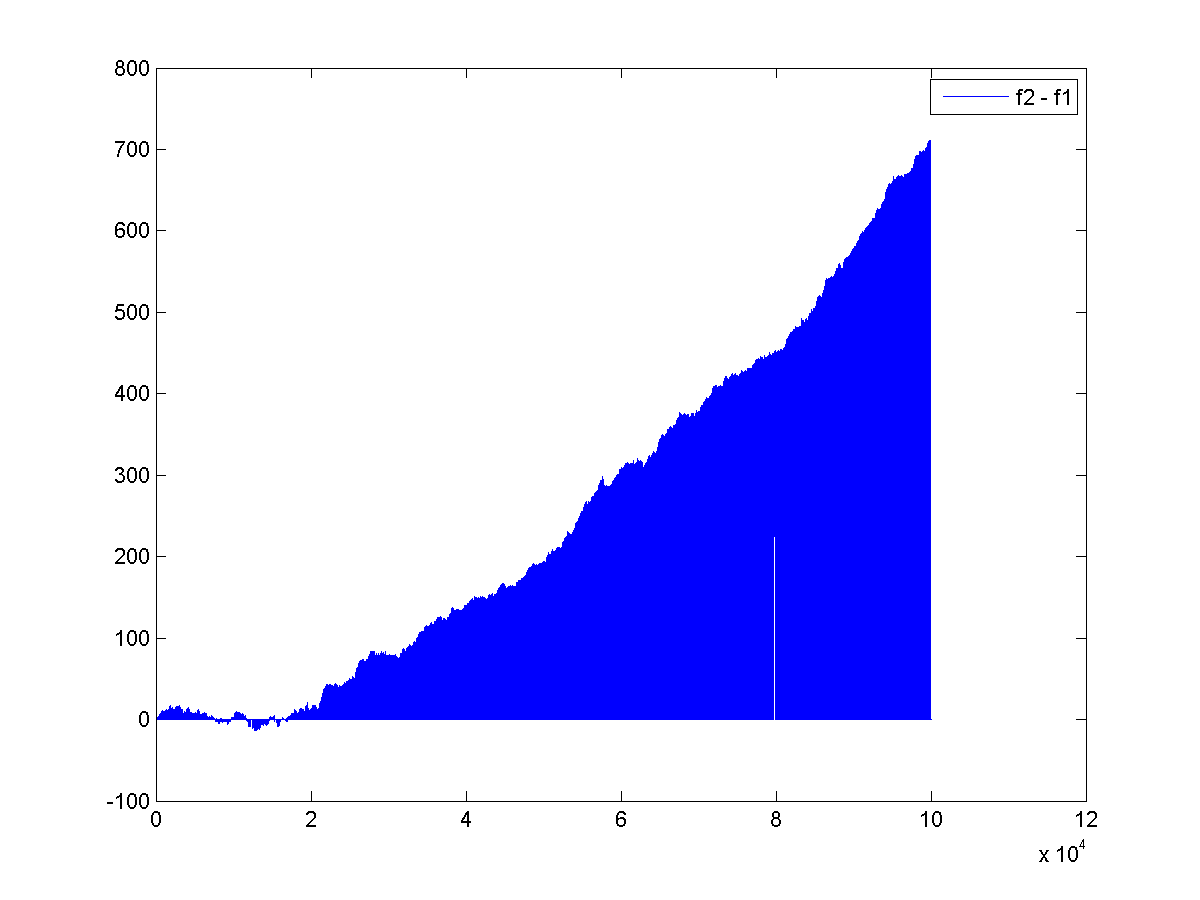
\includegraphics[scale=0.33]{Figures/base1/base3_1} 
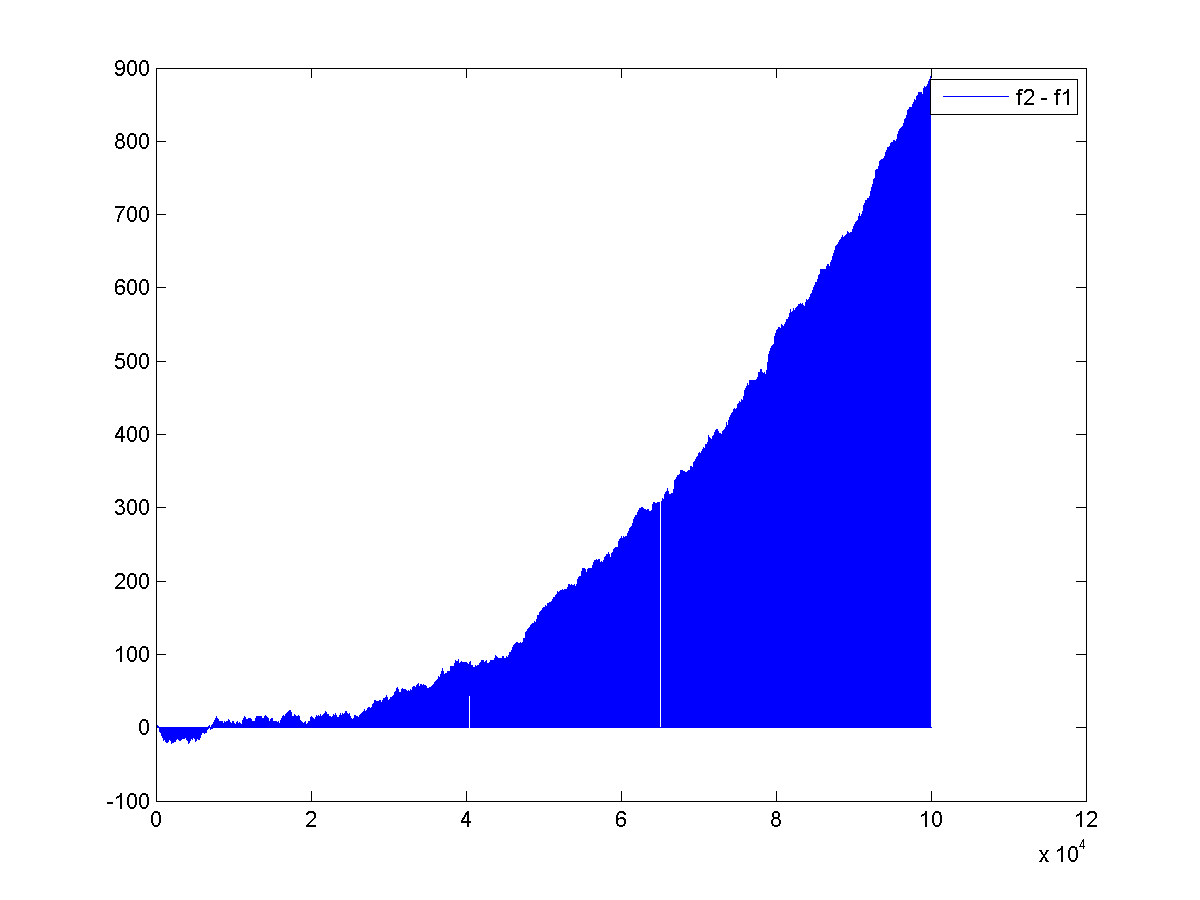
\includegraphics[scale=0.33]{Figures/base1/base3_2} \\
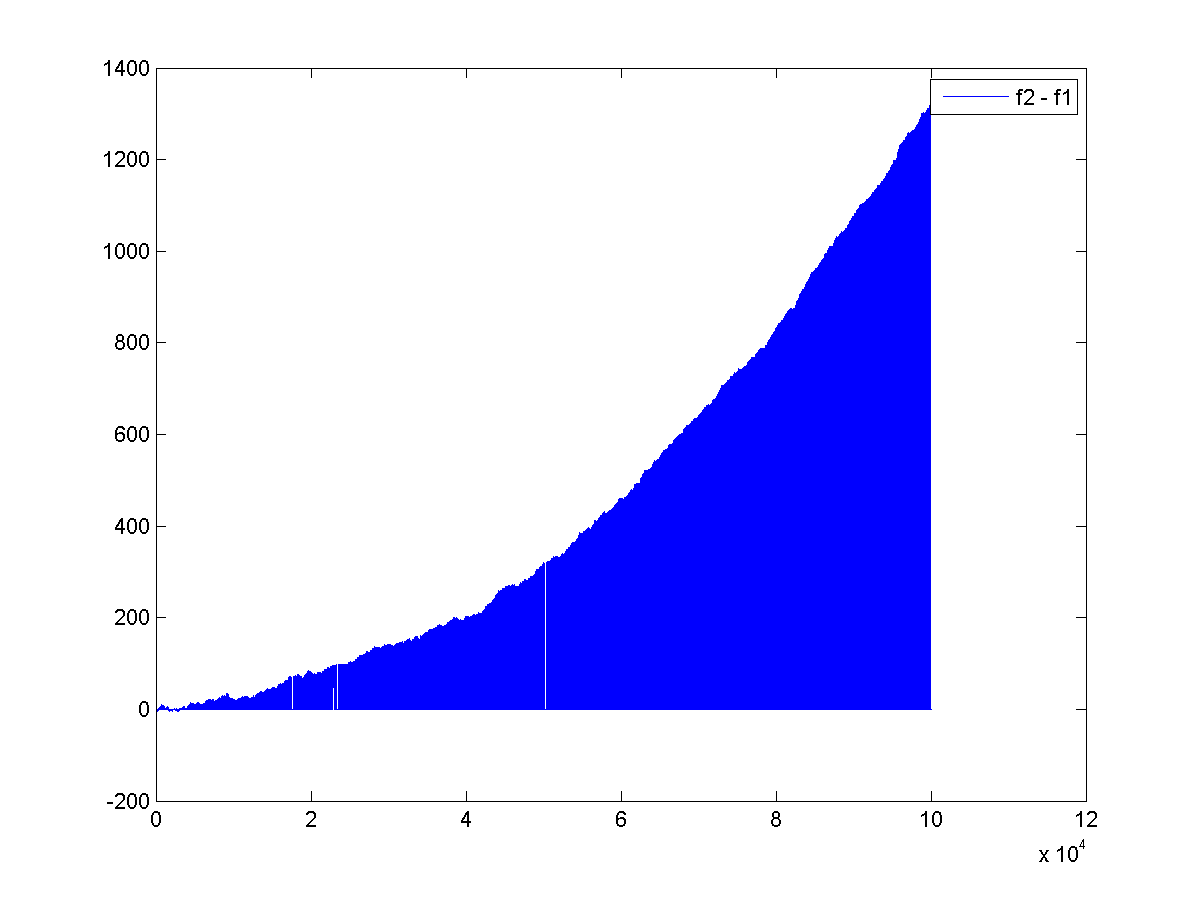
\includegraphics[scale=0.33]{Figures/base1/base3_3}
\end{array}$
\end{center}
\caption[Base case 3]{Results from three simulations for base case 3.}
\label{fig:base3}
\end{figure}

\begin{figure}
\begin{center}$
\begin{array}{ccc}
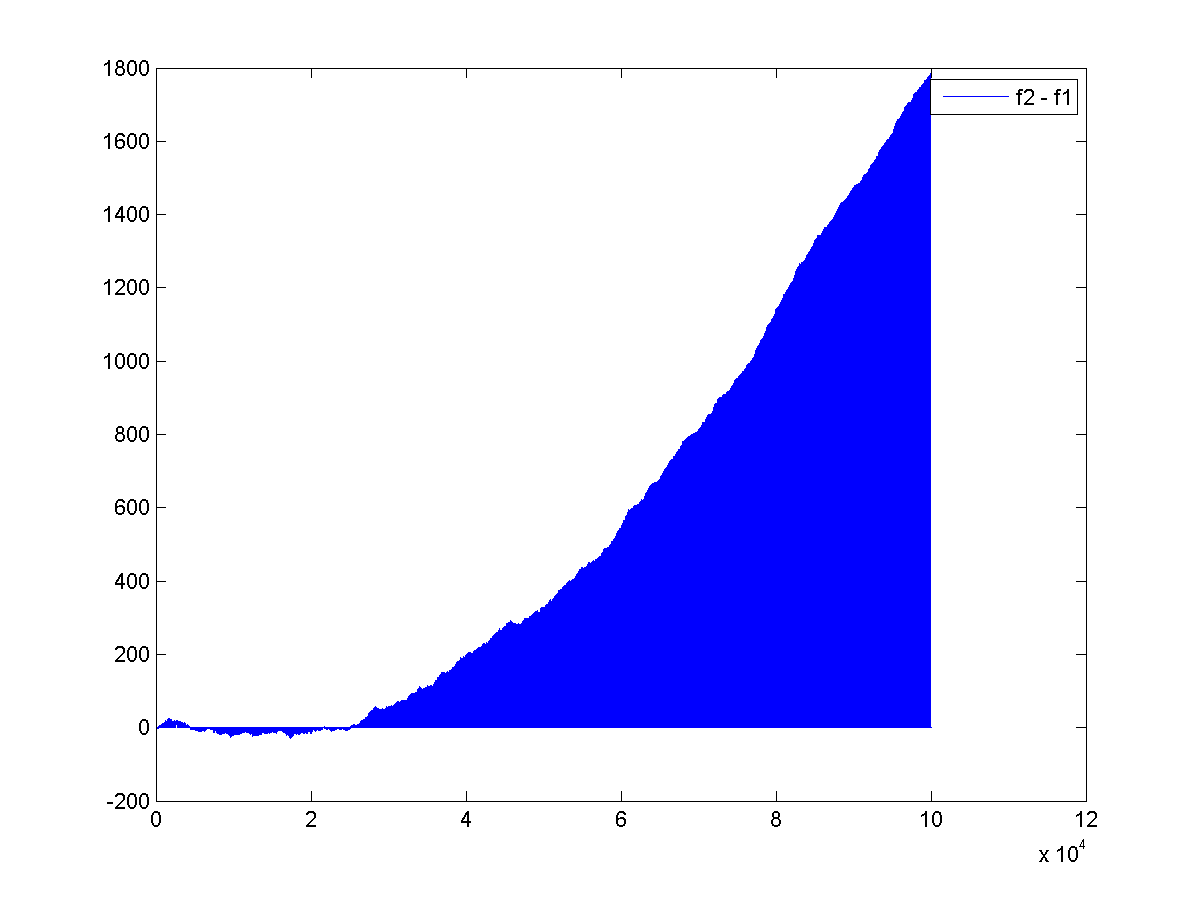
\includegraphics[scale=0.33]{Figures/base1/base4_1} 
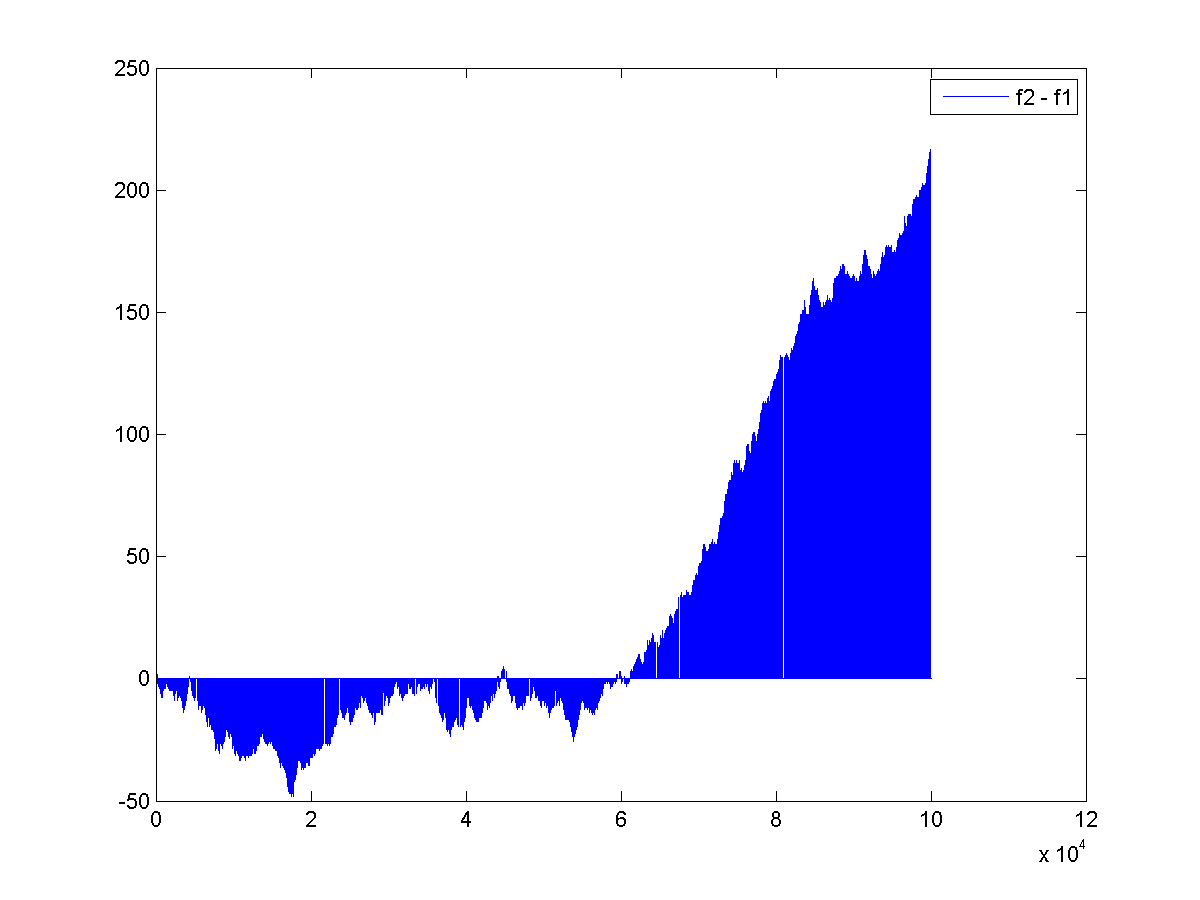
\includegraphics[scale=0.33]{Figures/base1/base4_2} \\
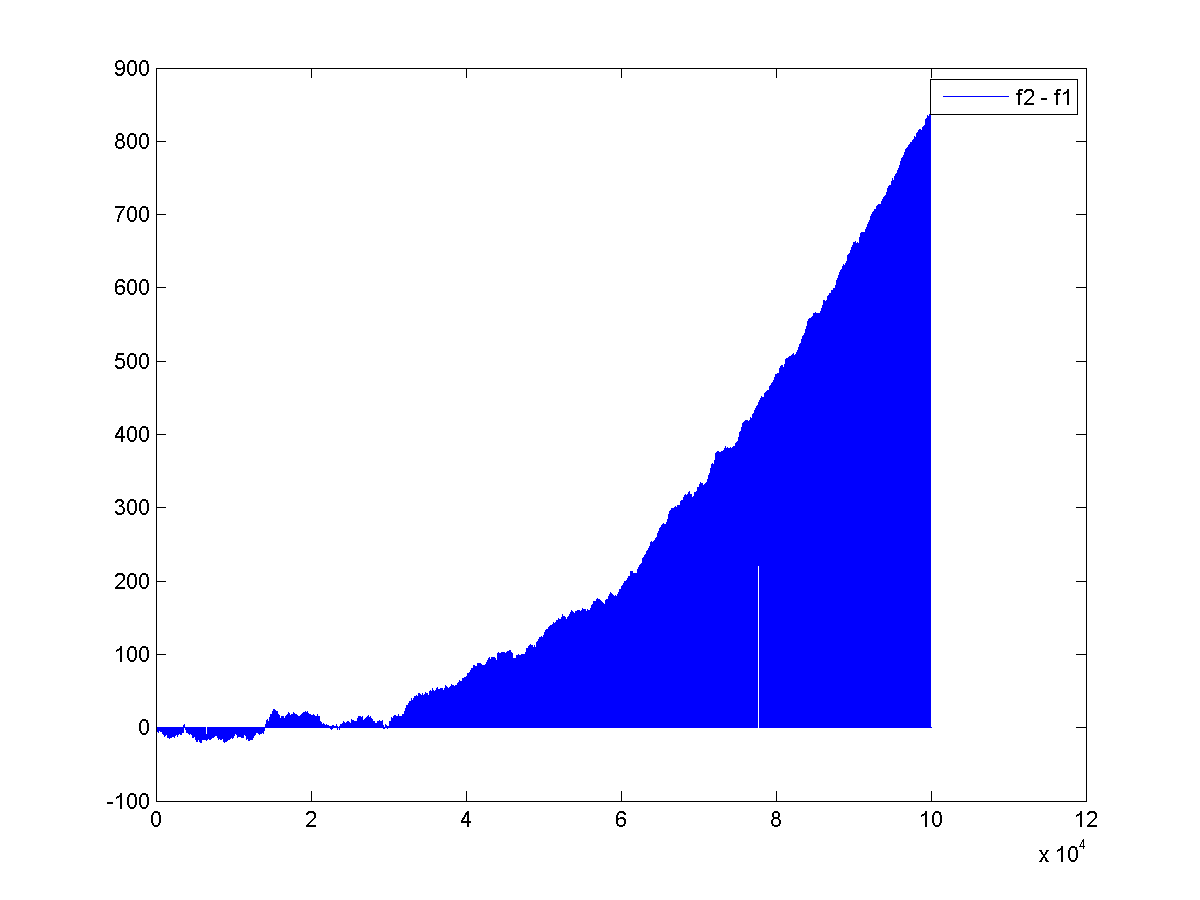
\includegraphics[scale=0.33]{Figures/base1/base4_3}
\end{array}$
\end{center}
\caption[Base case 4]{Results from three simulations for base case 4.}
\label{fig:base4}
\end{figure}

\begin{figure}
\begin{center}$
\begin{array}{ccc}
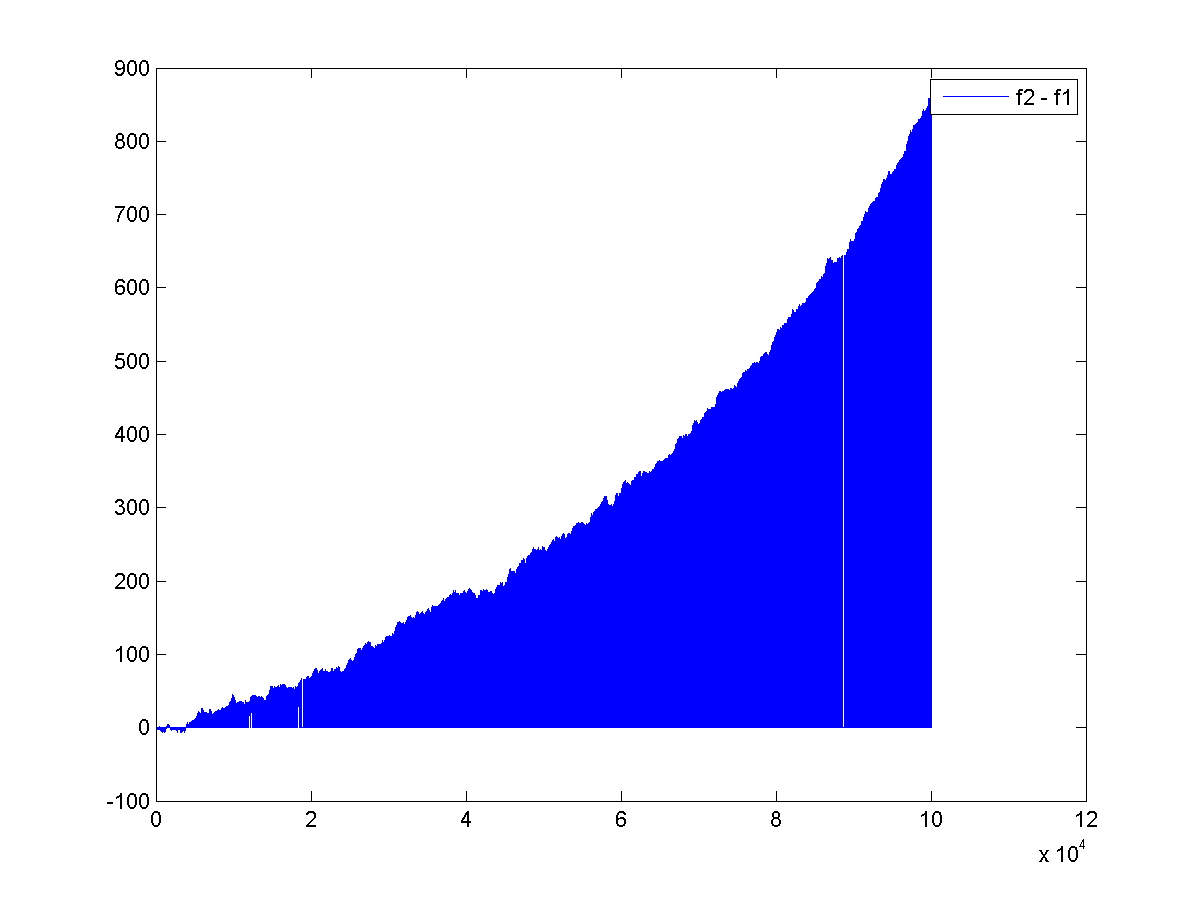
\includegraphics[scale=0.33]{Figures/base1/diff1_1} 
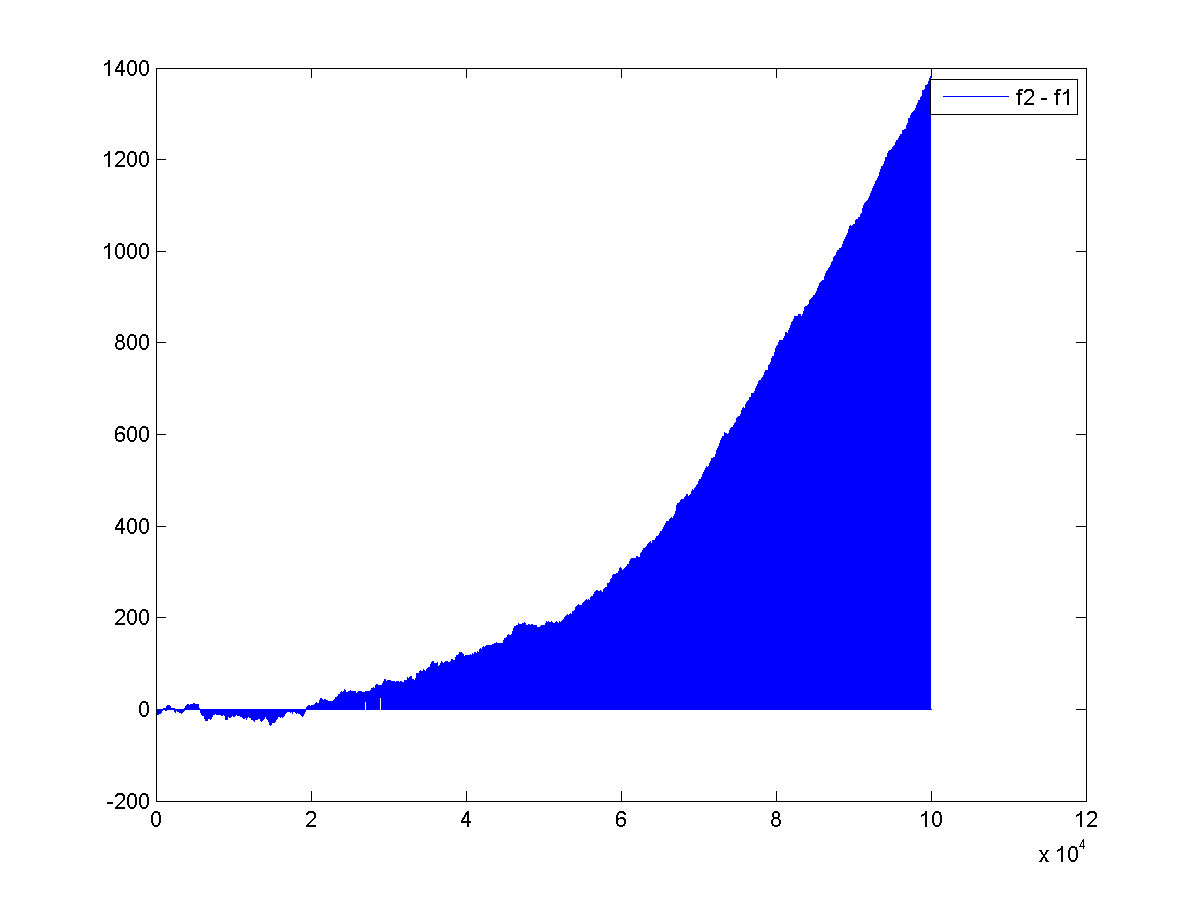
\includegraphics[scale=0.33]{Figures/base1/diff1_2} \\
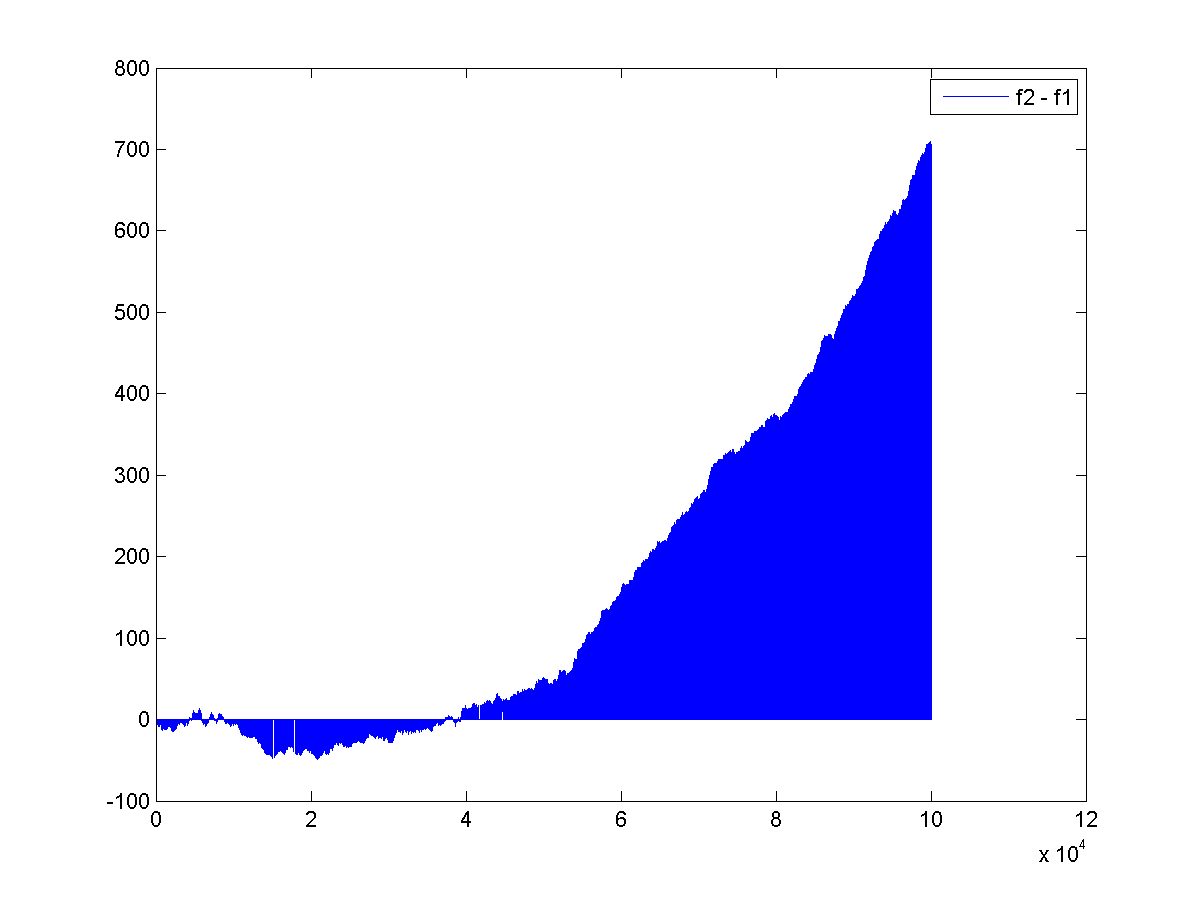
\includegraphics[scale=0.33]{Figures/base1/diff1_3}
\end{array}$
\end{center}
\caption[Difference case 1]{Results from three simulations for difference case 1.}
\label{fig:diff1}
\end{figure}

\begin{figure}
\begin{center}$
\begin{array}{ccc}
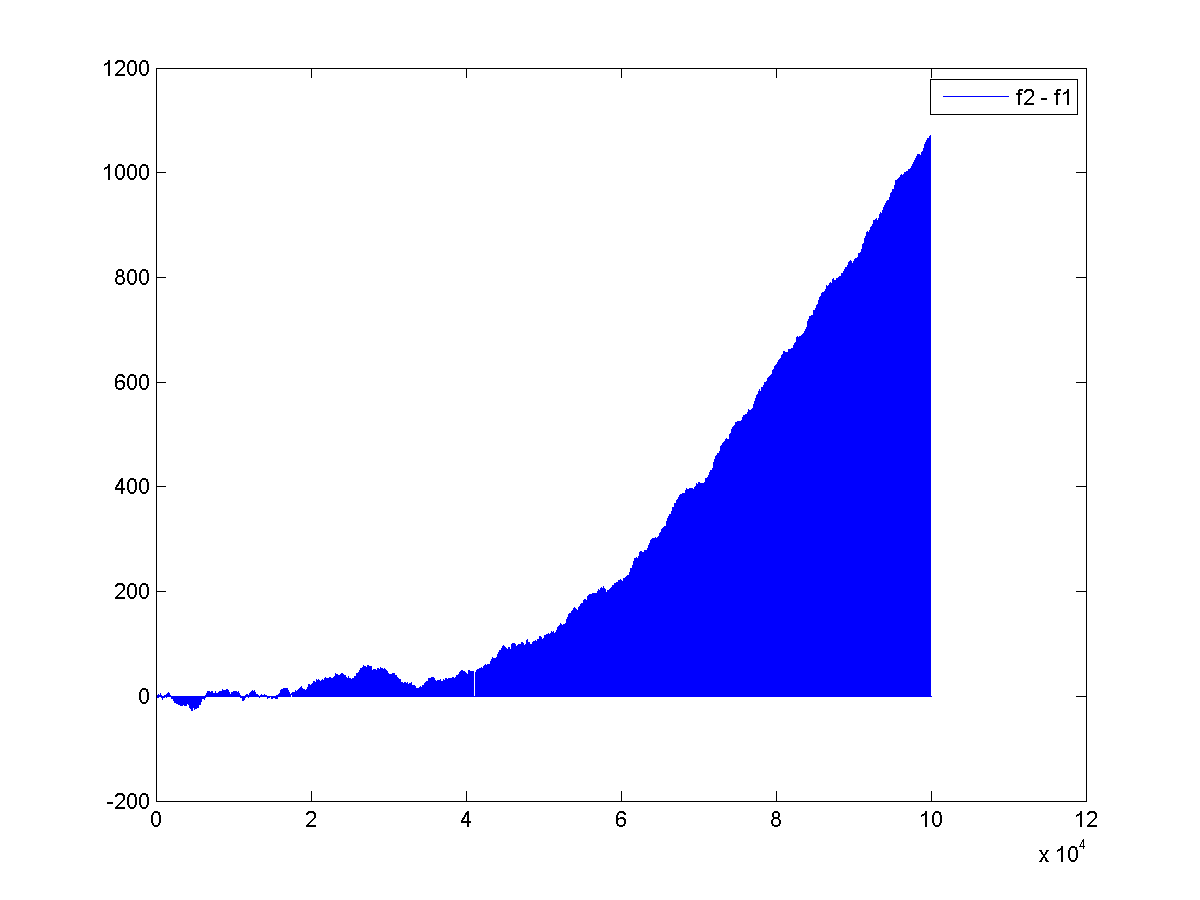
\includegraphics[scale=0.33]{Figures/base1/diff2_1} 
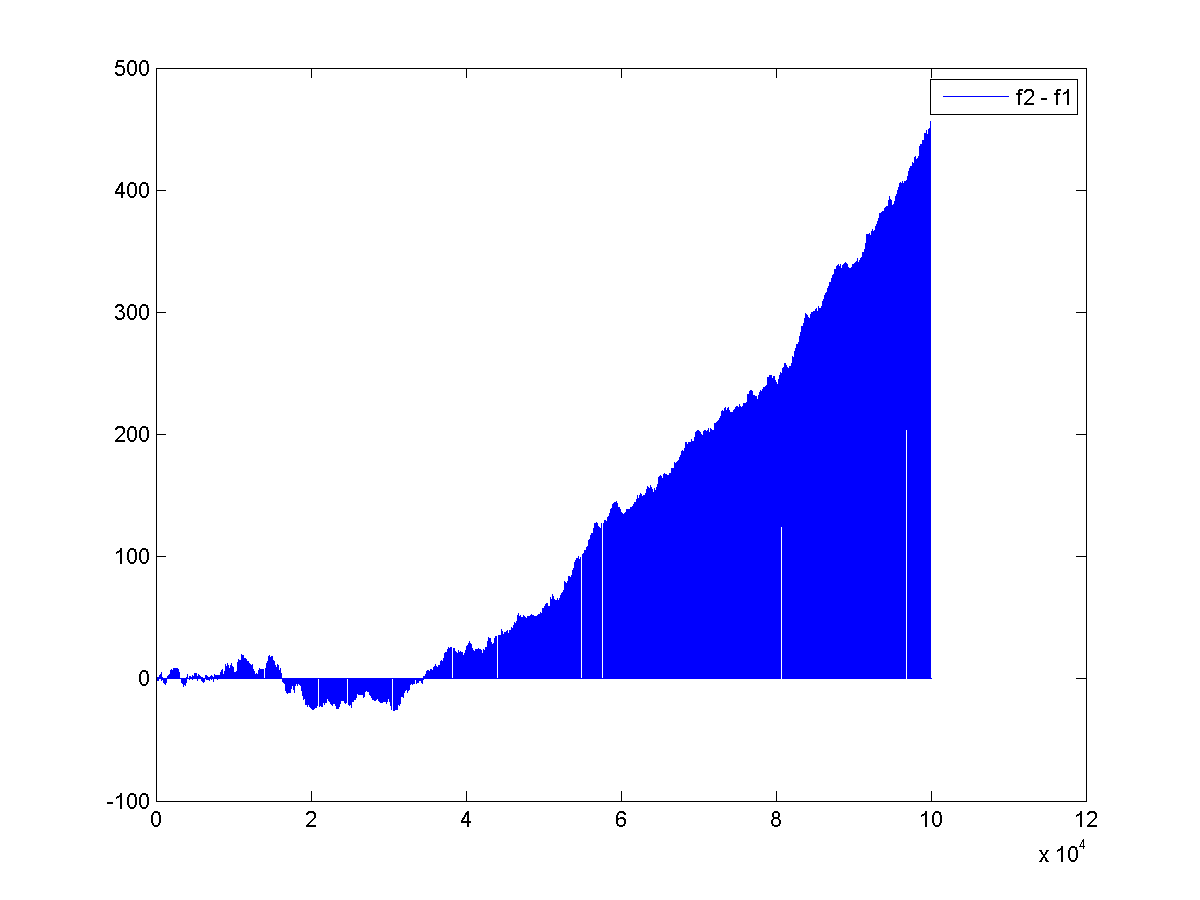
\includegraphics[scale=0.33]{Figures/base1/diff2_2} \\
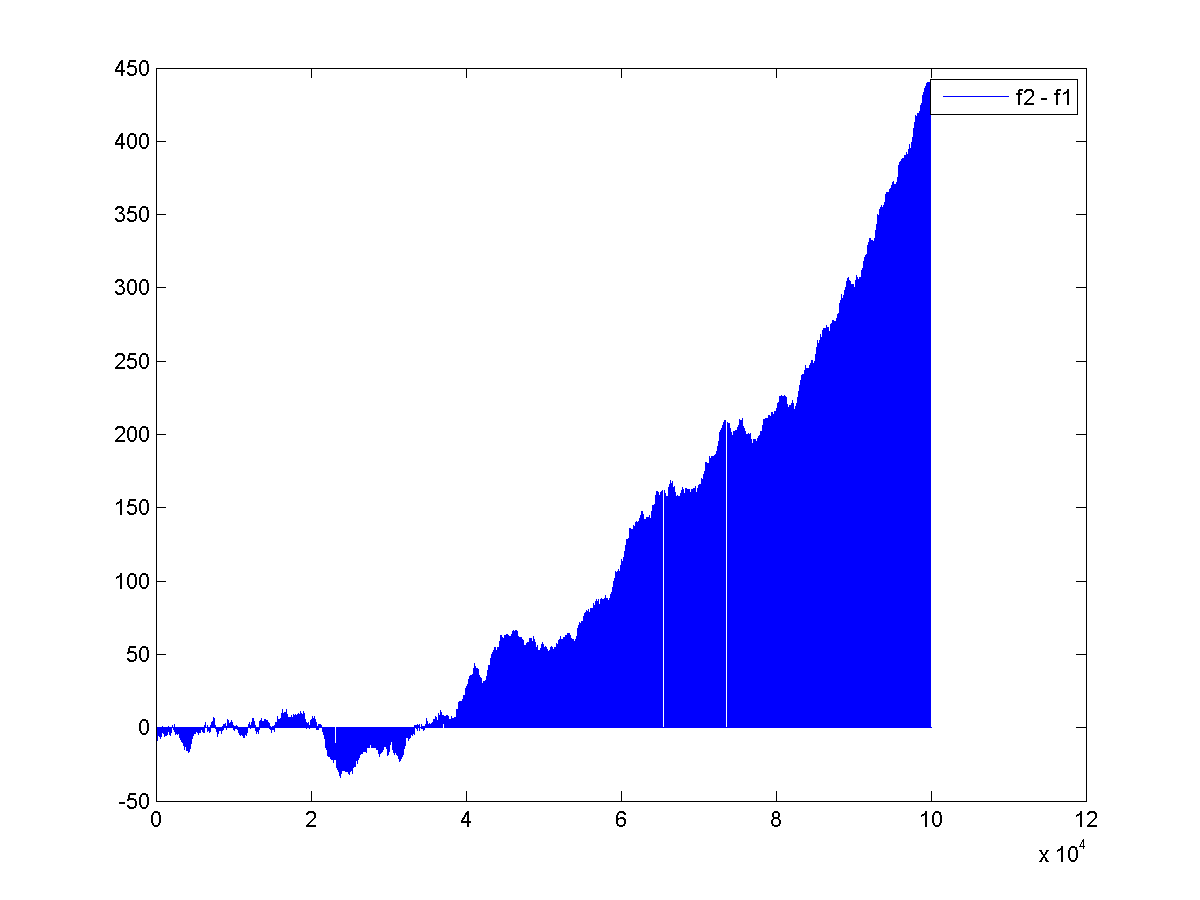
\includegraphics[scale=0.33]{Figures/base1/diff2_3}
\end{array}$
\end{center}
\caption[Difference case 2]{Results from three simulations for difference case 2.}
\label{fig:diff2}
\end{figure}

\begin{figure}
\begin{center}$
\begin{array}{ccc}
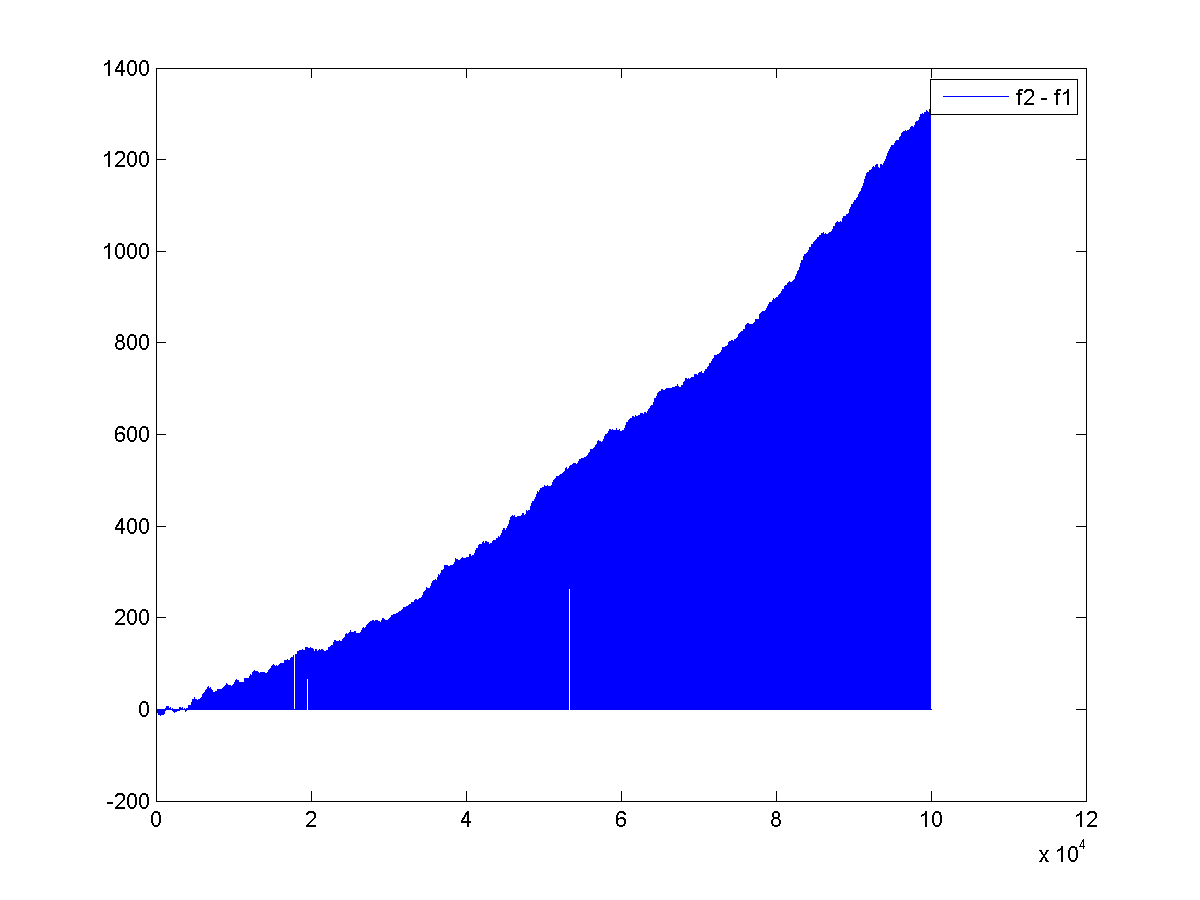
\includegraphics[scale=0.33]{Figures/base1/diff3_1} 
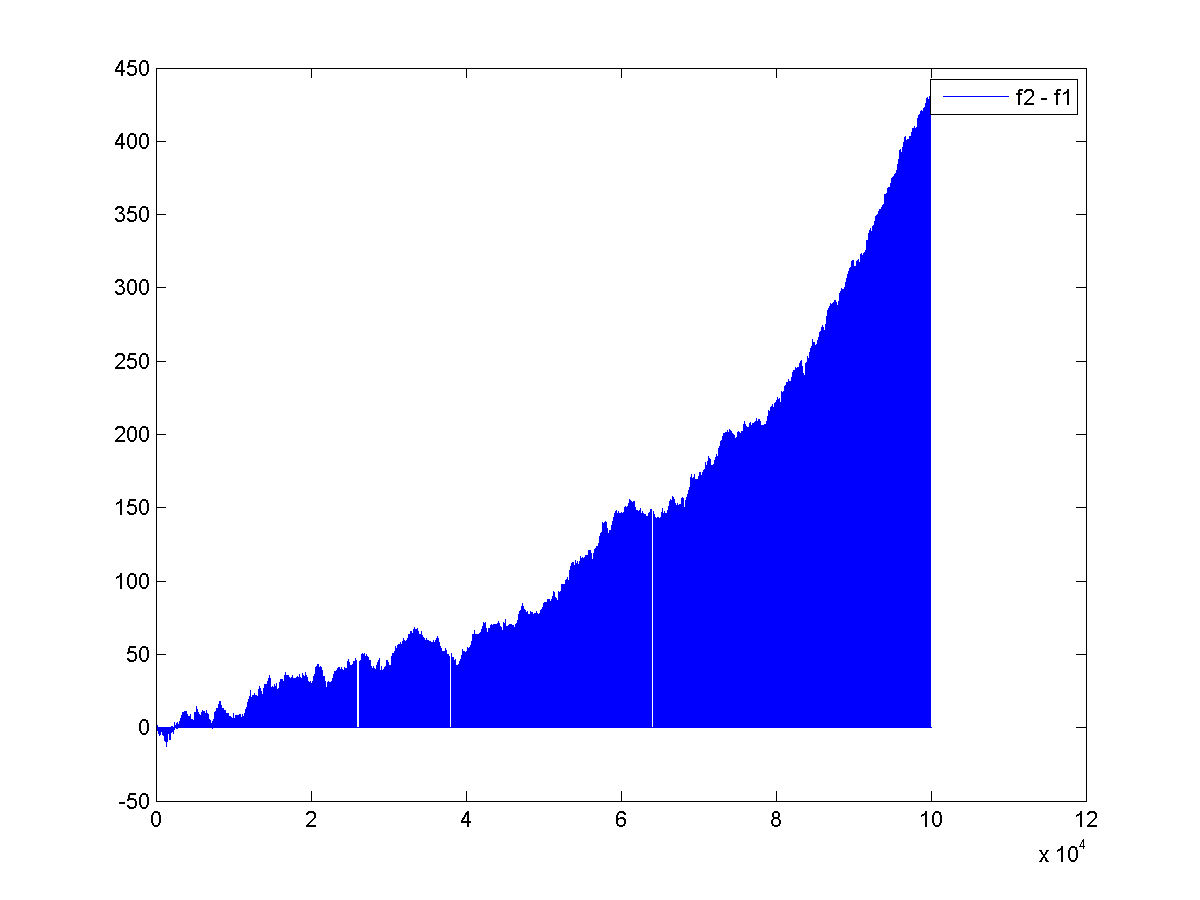
\includegraphics[scale=0.33]{Figures/base1/diff3_2} \\
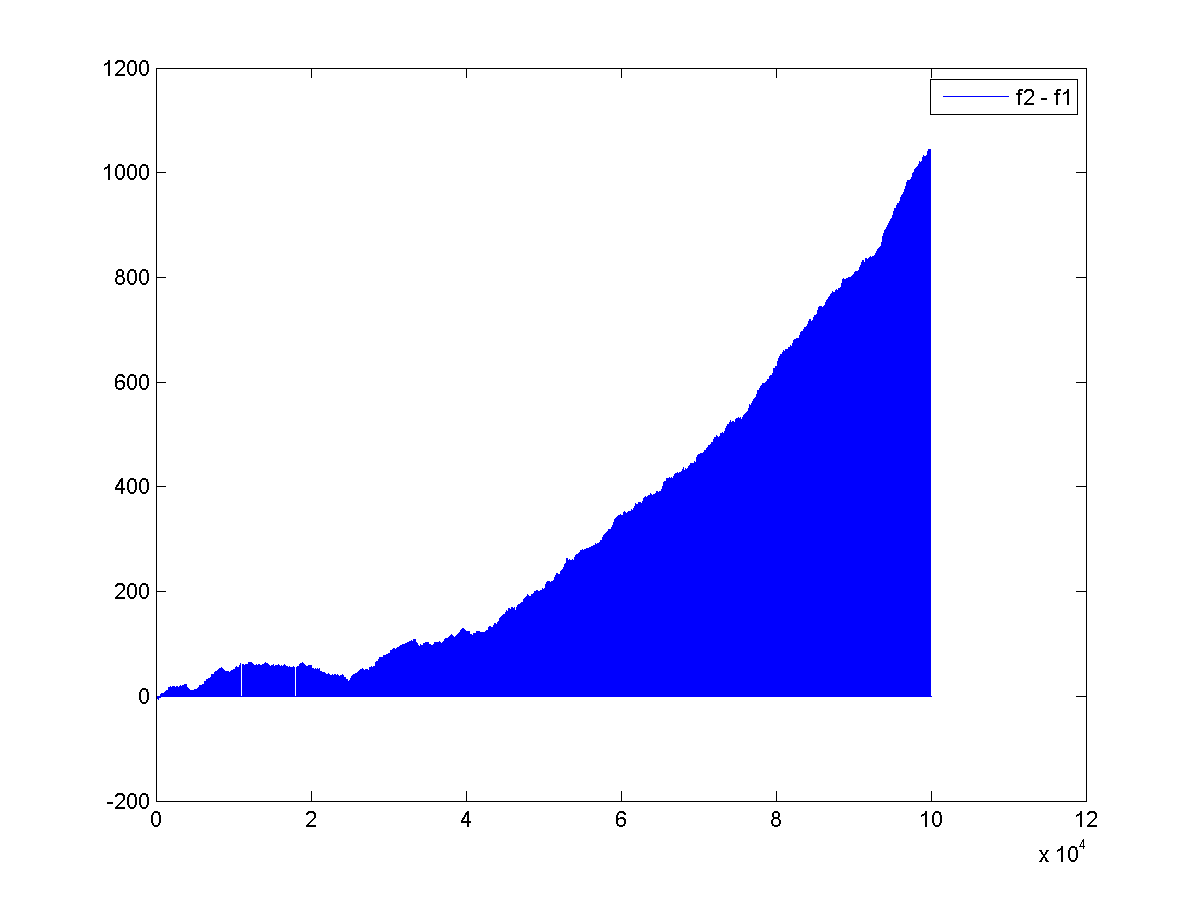
\includegraphics[scale=0.33]{Figures/base1/diff3_3}
\end{array}$
\end{center}
\caption[Difference case 3]{Results from three simulations for difference case 3.}
\label{fig:diff3}
\end{figure}

\begin{figure}
\begin{center}$
\begin{array}{ccc}
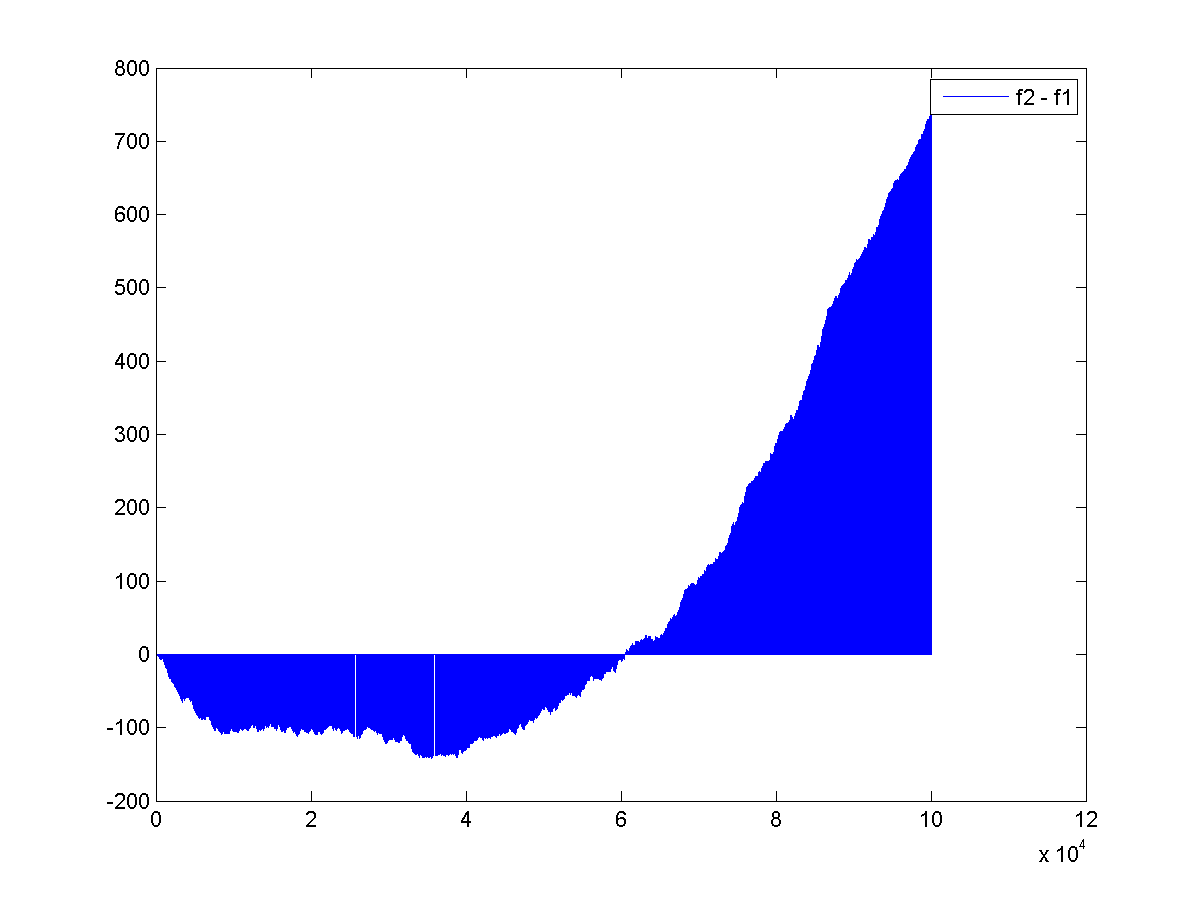
\includegraphics[scale=0.33]{Figures/base1/diff4_1} 
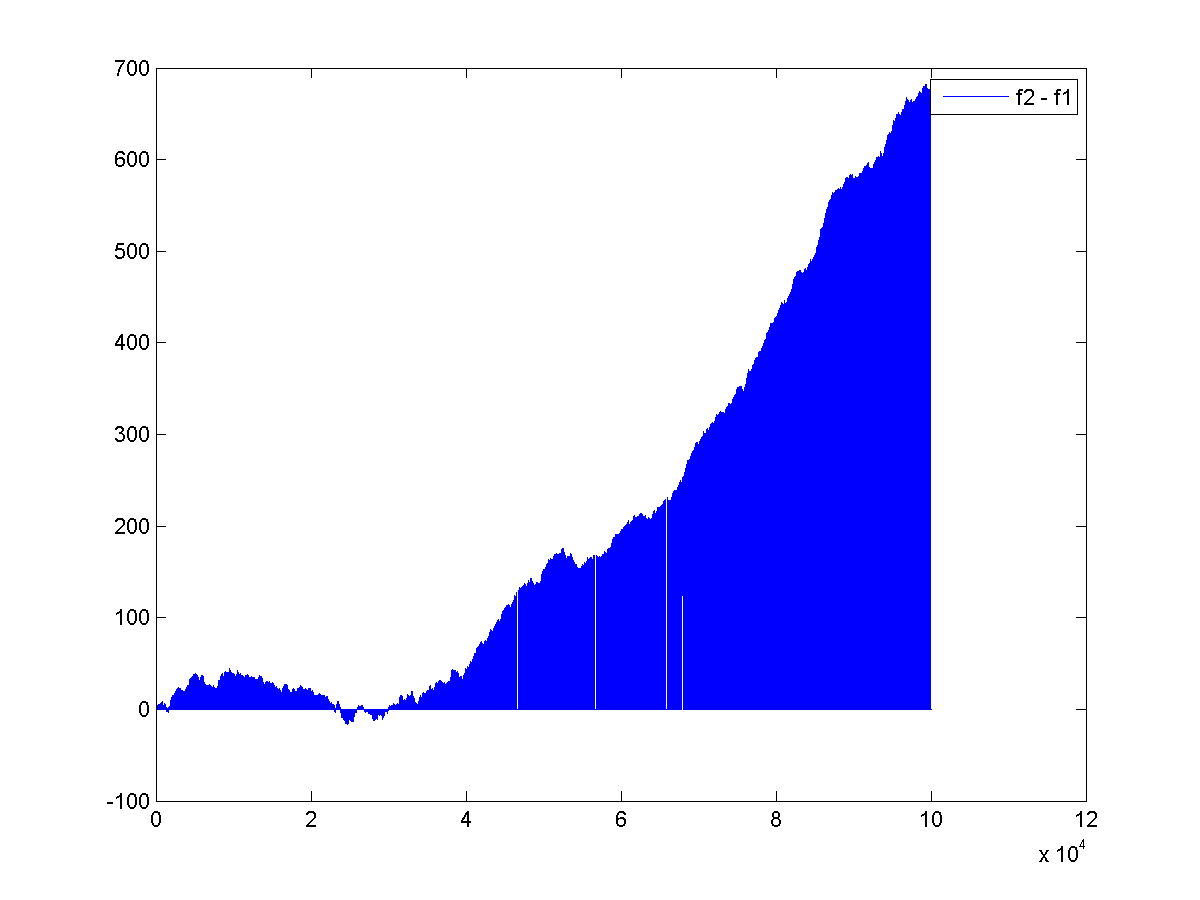
\includegraphics[scale=0.33]{Figures/base1/diff4_2} \\
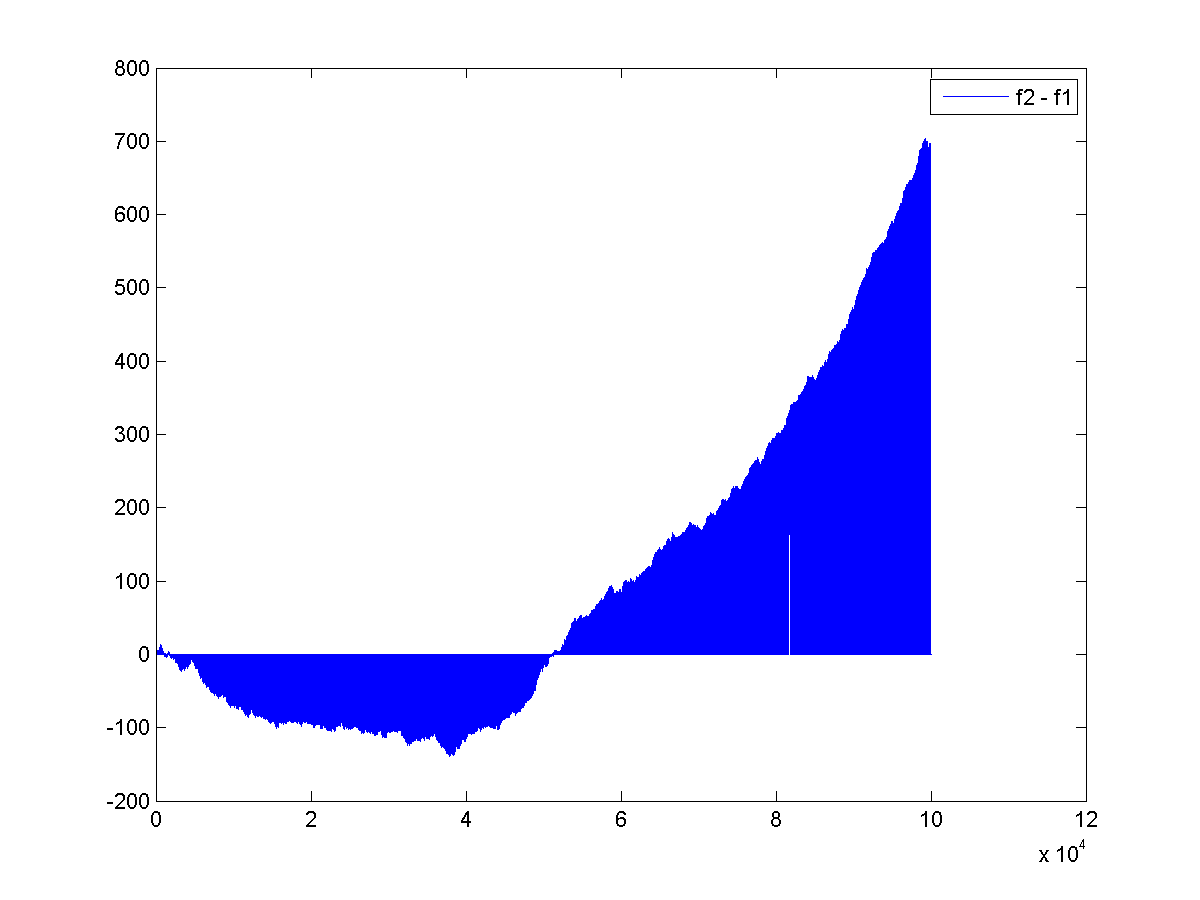
\includegraphics[scale=0.33]{Figures/base1/diff4_3}
\end{array}$
\end{center}
\caption[Difference case 4]{Results from three simulations for difference case 4.}
\label{fig:diff4}
\end{figure}

\begin{figure}
\begin{center}$
\begin{array}{ccc}
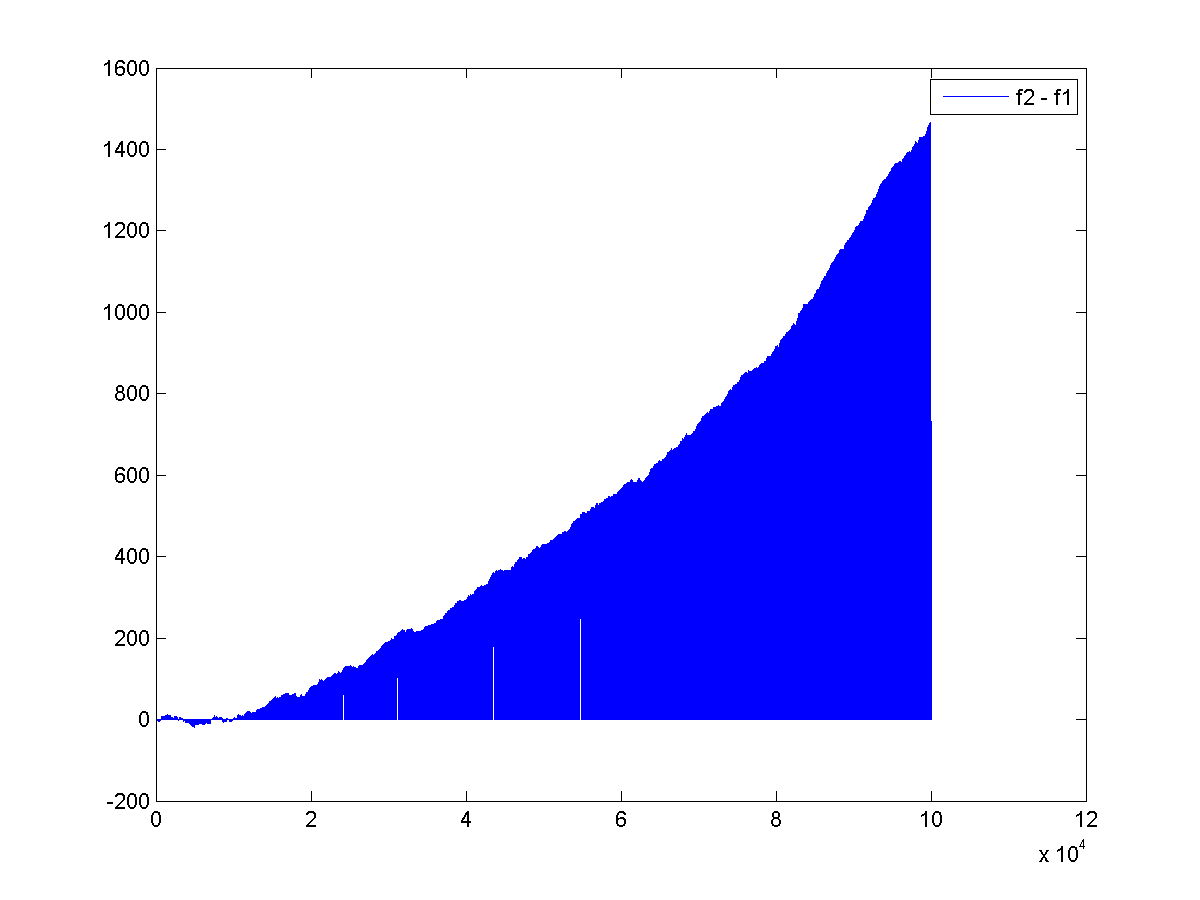
\includegraphics[scale=0.33]{Figures/base1/diff5_1} 
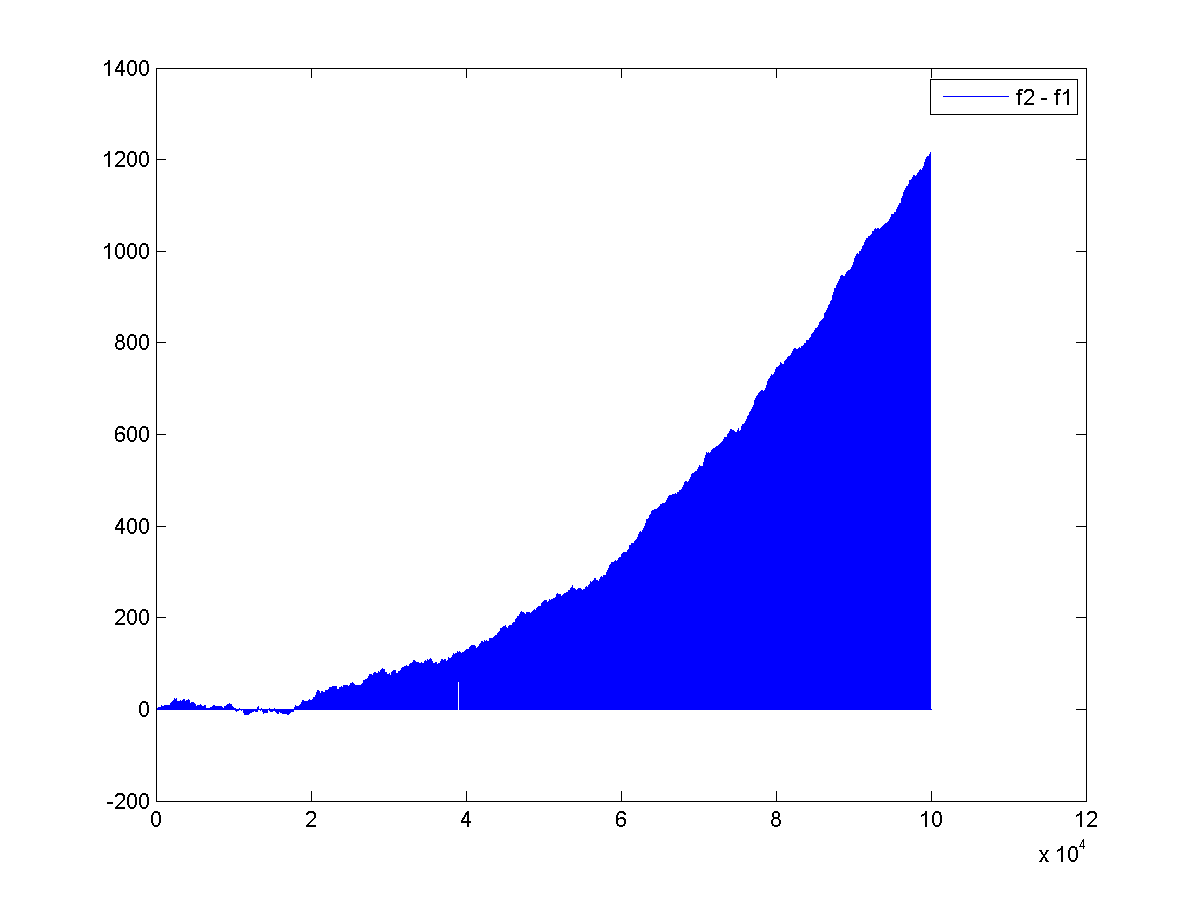
\includegraphics[scale=0.33]{Figures/base1/diff5_2} \\
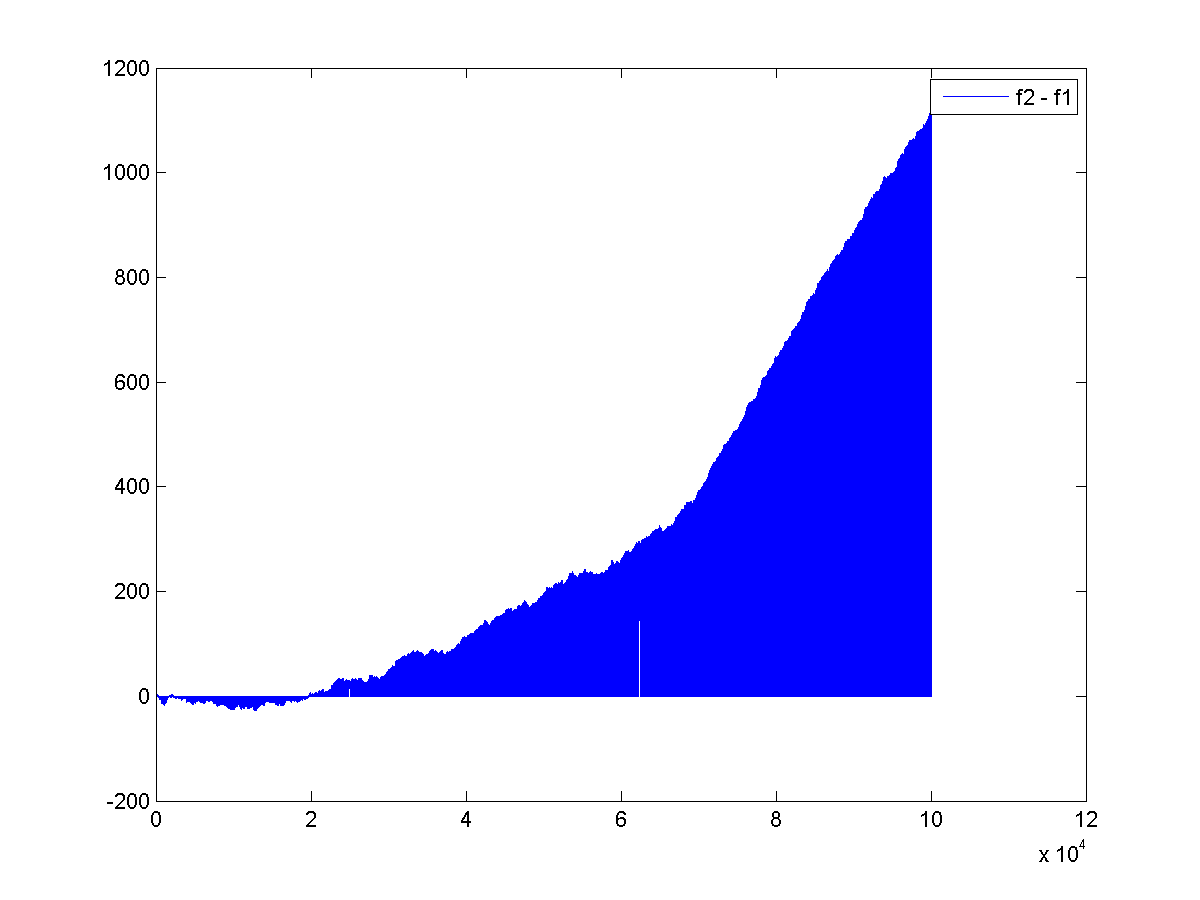
\includegraphics[scale=0.33]{Figures/base1/diff5_3}
\end{array}$
\end{center}
\caption[Difference case 5]{Results from three simulations for difference case 5.}
\label{fig:diff5}
\end{figure}

\begin{figure}
\begin{center}$
\begin{array}{ccc}
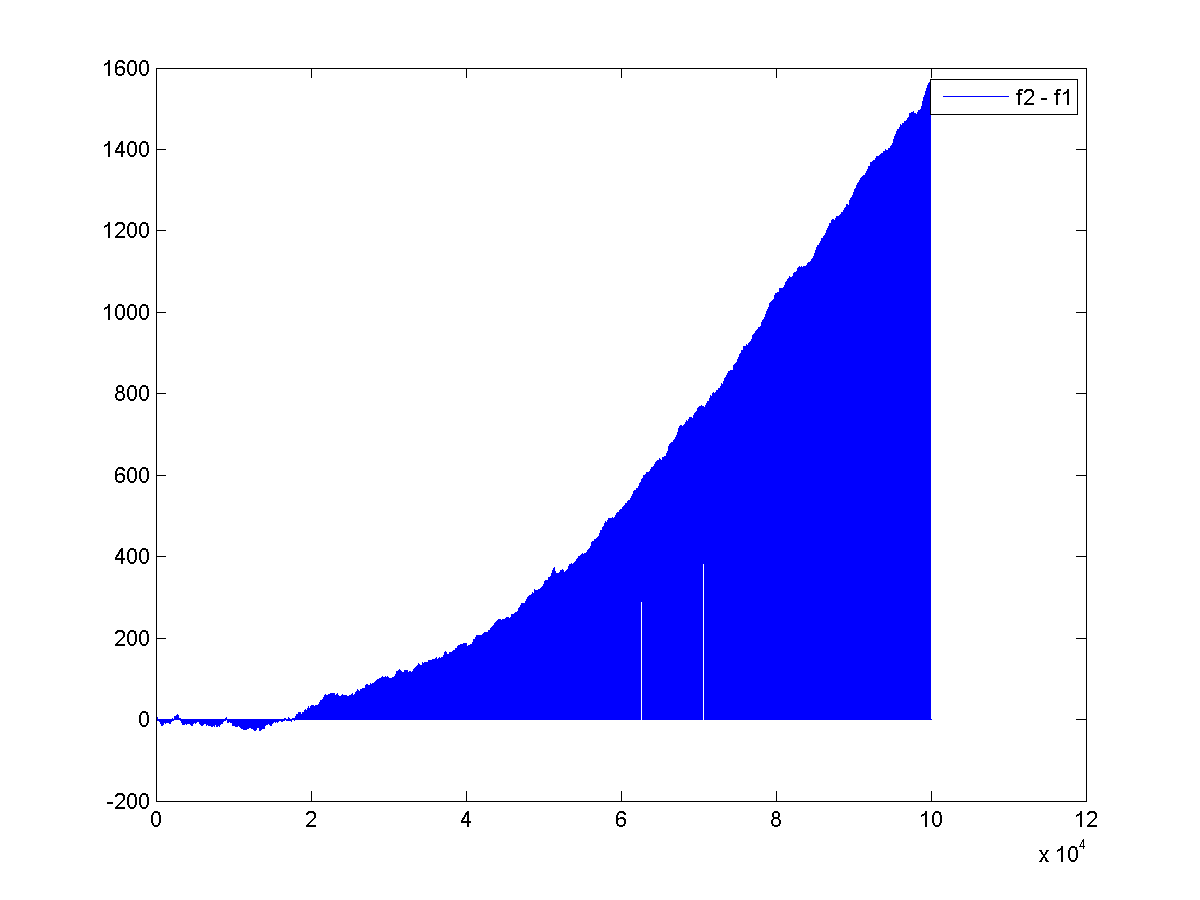
\includegraphics[scale=0.33]{Figures/base1/diff6_1} 
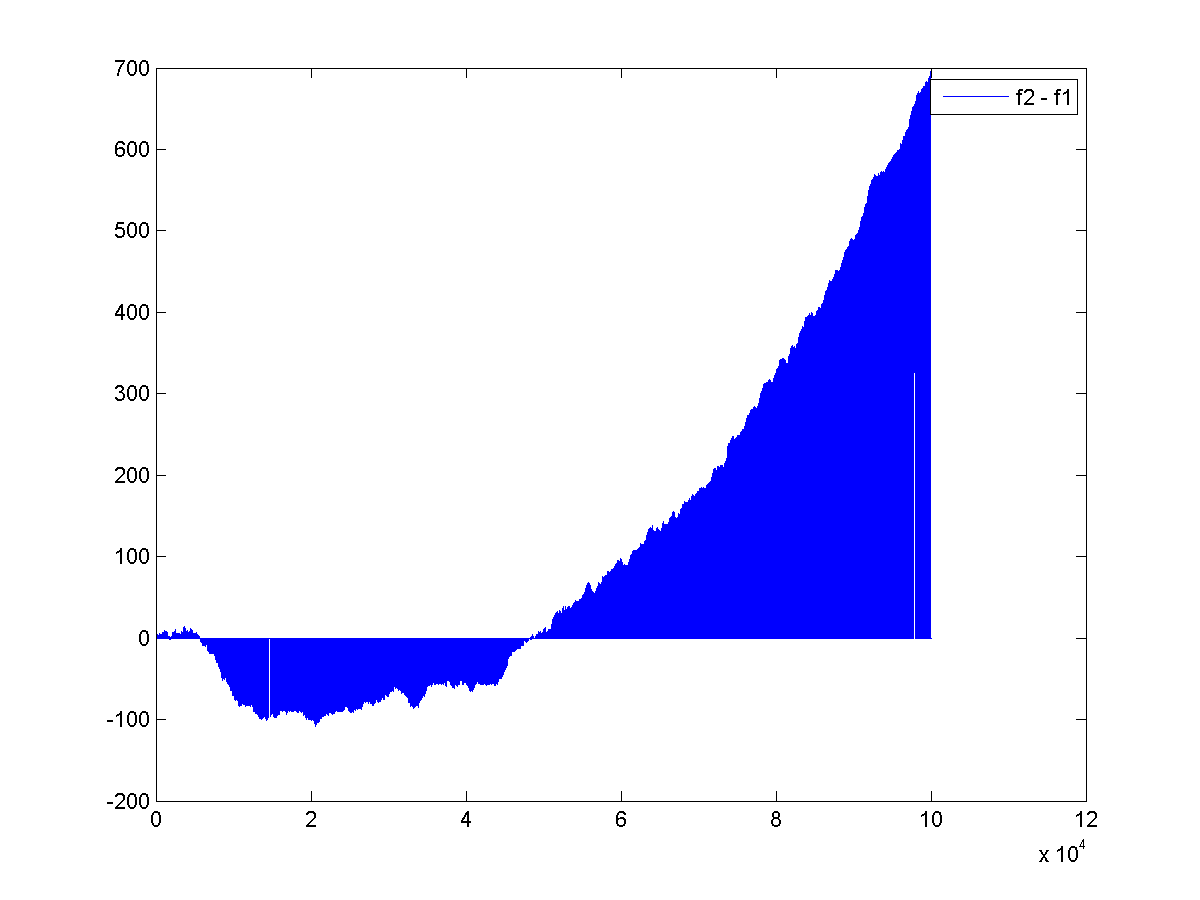
\includegraphics[scale=0.33]{Figures/base1/diff6_2} \\
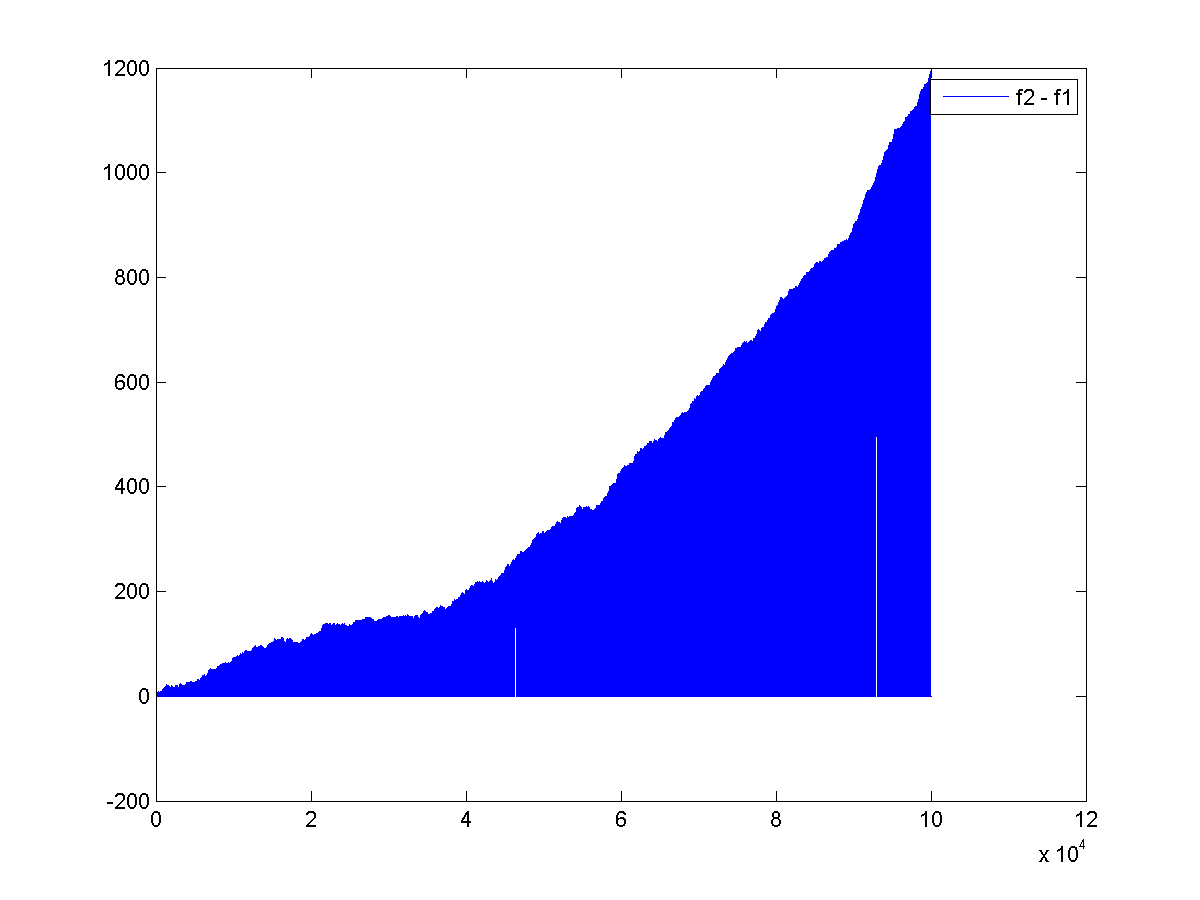
\includegraphics[scale=0.33]{Figures/base1/diff6_3}
\end{array}$
\end{center}
\caption[Difference case 6]{Results from three simulations for difference case 6.}
\label{fig:diff6}
\end{figure}